\chapter{Protocolos de comunicação}
\label{chap:background}

Este capítulo apresenta os conceitos e os protocolos de comunicação que fundamentam a solução proposta neste trabalho, a qual implementa o QUIC sobre uma infraestrutura baseada em WebRTC. O capítulo está organizado da seguinte forma: \cfm{tive que organizar uma introdução}

\begin{itemize}

\item A Seção \ref{sec:protocol_stack} situa os protocolos abordados nos modelos de referência OSI (\textit{Open Systems Interconnection}) e TCP/IP (\textit{Transmission Control Protocol/Internet Protocol}) e delimita as camadas de rede e de transporte como foco do trabalho.

\item A Seção \ref{sec:network_architecture_models} apresenta os modelos arquiteturais de rede --- cliente-servidor, \textit{peer-to-peer} e híbrido --- e sua relação com a solução proposta.

\item A Seção \ref{sec:network_address_translator} descreve o funcionamento do NAT, suas características e classificações, bem como o problema que ele impõe à comunicação P2P.

\item A Seção \ref{sec:nat_traversal} expõe as técnicas de travessia de NAT, incluindo \textit{relaying}, \textit{connection reversal} e \textit{hole punching} sobre UDP e TCP.

\item A Seção \ref{sec:ice} apresenta o protocolo ICE e os servidores STUN e TURN empregados na descoberta e seleção de candidatos de comunicação.

\item A Seção \ref{sec:chownat} detalha a arquitetura e o protocolo Chownat, incluindo os tipos de pacotes e as etapas de conexão e comunicação.
\item A Seção \ref{sec:webrtc} descreve a arquitetura e o protocolo WebRTC, abrangendo sinalização, estabelecimento de conexão, segurança e a API (\textit{Application Programming Interface}).

% \item A Seção \ref{sec:quic} apresenta o protocolo QUIC, sua motivação em relação ao TCP e seu uso em aplicações P2P, incluindo cenários de tempo real e IoT.

\end{itemize}

O protocolo QUIC também integra a pilha de protocolos de comunicação; entretanto, devido à sua complexidade e relevância para este trabalho, o Capítulo~\ref{chap:quic} o aborda separadamente.

%%%%%%%%%%%%%%%%%%%%%%%%%%%%%%%%%%%%%%%%%%%%%%%%%%%%%%%%%%%%%%%%%%%%%%%%%%%%%%%%%%%
% OSI AND TCP/IP STACK
%%%%%%%%%%%%%%%%%%%%%%%%%%%%%%%%%%%%%%%%%%%%%%%%%%%%%%%%%%%%%%%%%%%%%%%%%%%%%%%%%%%
\section{Relações da Pilha de Protocolos}
\label{sec:protocol_stack}

Para compreender a relação entre os protocolos abordados neste trabalho, é necessário entender como eles se organizam nas pilhas de rede. O modelo OSI \citep{iso7498} define uma referência de sete camadas, que serve como abstração para a organização das funções de comunicação em redes. Posteriormente, consolidou-se a arquitetura de protocolos da Internet, comumente denominada arquitetura TCP/IP, que organiza as funções de comunicação em quatro camadas \citep{rfc1122}. Modelos de cinco camadas também representam essa arquitetura, principalmente para distinguir as funções das camadas de enlace e física. Este trabalho adota o modelo de cinco camadas como referência. A Figura~\ref{fig:osi_tcpip} apresenta essas camadas e suas correspondências com o modelo OSI.

\begin{figure}[!ht]
        \centering
        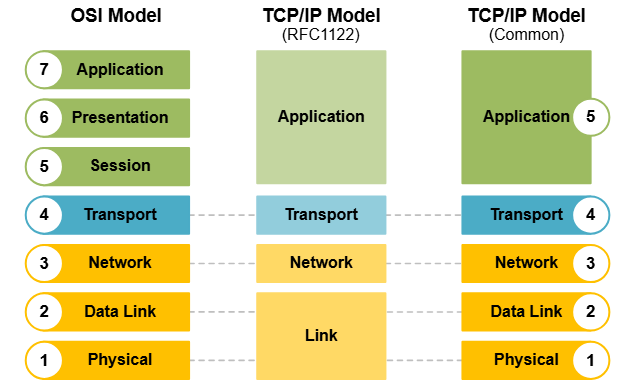
\includegraphics[width=0.7\linewidth]{fig/relationship/osi_tcpip.png}
        \caption{Comparação entre os modelos OSI e TCP/IP por \citep{networkacademy2026osi}.}
        \label{fig:osi_tcpip}
\end{figure}

Este trabalho concentra-se nas camadas de rede e de transporte, correspondentes às camadas 3 e 4 do modelo OSI. A camada de rede é responsável pelo endereçamento e pelo encaminhamento de pacotes entre diferentes redes, enquanto a camada de transporte é responsável pela comunicação fim a fim entre os \textit{peers}. Na arquitetura TCP/IP, essas funções correspondem, respectivamente, às camadas de Internet (\textit{Internet layer}) e de transporte (\textit{transport layer}) \citep{rfc1122}.

Este trabalho utiliza uma infraestrutura baseada em WebRTC, descrita na Seção~\ref{sec:webrtc}. Nessa infraestrutura, a comunicação entre os \textit{peers} depende dos mecanismos de travessia de NAT, descritos na Seção~\ref{sec:nat_traversal}, e do protocolo ICE, apresentado na Seção~\ref{sec:ice}, que realiza a descoberta e a seleção de candidatos de conexão. Sobre essa infraestrutura, o QUIC, descrito no Capítulo~\ref{chap:quic}, atua como protocolo de transporte e encapsula a comunicação TCP entre os \textit{peers}.

A arquitetura considerada neste trabalho é composta por dois \textit{peers} e por servidores auxiliares empregados pelos mecanismos de travessia de NAT. Cada \textit{peer} é um \textit{gateway} associado a um dispositivo IoT ou a uma aplicação consumidora dos dados gerados por esse dispositivo, representados na figura como \textit{device1} e \textit{device2}. Essa aplicação pode ser executada em um sistema de propósito geral ou em outro dispositivo IoT. Os \textit{gateways} executam a infraestrutura proposta e são distintos dos roteadores de acesso, responsáveis pelo encaminhamento dos pacotes e pela tradução de endereços nas redes representadas. As aplicações locais assumem os papéis de cliente e servidor, enquanto os \textit{gateways} viabilizam a comunicação entre elas.

A Figura~\ref{fig:quic_p2p_architecture} apresenta a arquitetura de comunicação proposta neste trabalho, com seus principais elementos e as relações entre eles. Este capítulo descreve os fundamentos teóricos das operações realizadas entre os \textit{peers}, os servidores e os demais elementos da arquitetura, e o Capítulo~\ref{chap:implementation} apresenta a implementação prática dessas operações.

\begin{figure}[!ht]
        \centering
        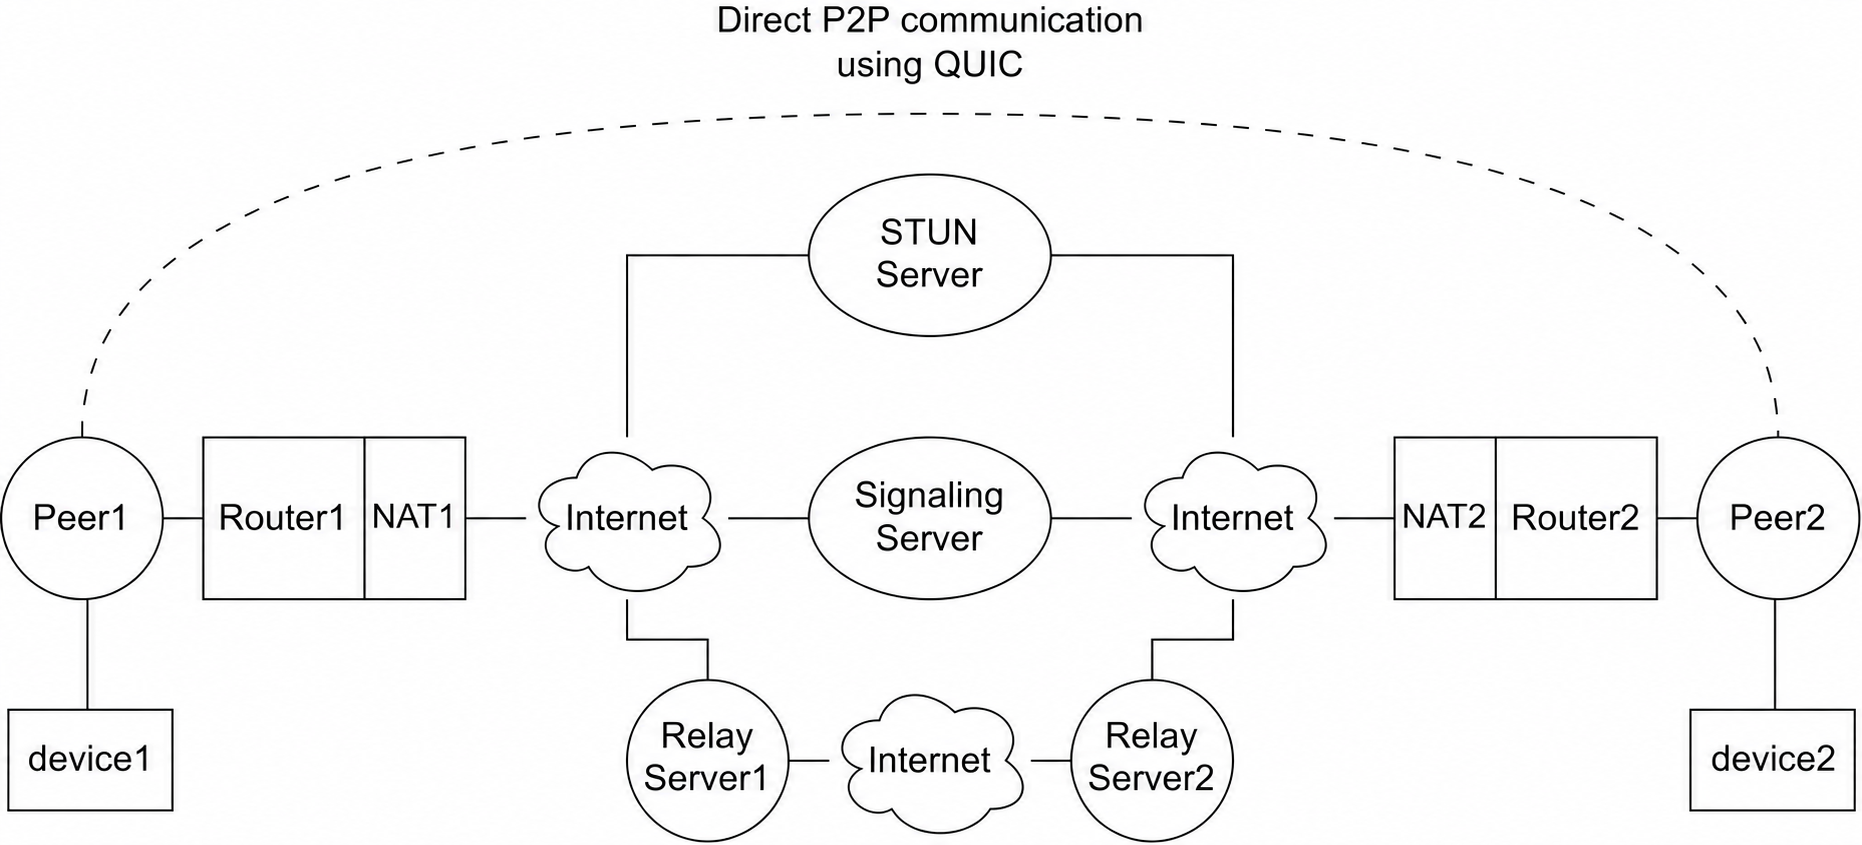
\includegraphics[width=1.0\linewidth]{fig/relationship/architecture_for_quic_p2p.png}
        \caption{Arquitetura para comunicação P2P com QUIC.}
        \label{fig:quic_p2p_architecture}
\end{figure}


%%%%%%%%%%%%%%%%%%%%%%%%%%%%%%%%%%%%%%%%%%%%%%%%%%%%%%%%%%%%%%%%%%%%%%%%%%%%%%%%%%%
% P2P NETWORKS
%%%%%%%%%%%%%%%%%%%%%%%%%%%%%%%%%%%%%%%%%%%%%%%%%%%%%%%%%%%%%%%%%%%%%%%%%%%%%%%%%%%
\section{Modelos de Arquitetura de Rede}
\label{sec:network_architecture_models}

O modelo de arquitetura de rede define a forma como os participantes de uma comunicação interagem entre si e os papéis que desempenham durante a prestação de um serviço. Esse modelo é frequentemente confundido com a topologia da rede, mas os conceitos são distintos: a arquitetura descreve o comportamento e as responsabilidades dos participantes, enquanto a topologia define como os dispositivos estão interconectados, seja física ou logicamente. Dessa forma, uma mesma arquitetura pode operar sobre diferentes topologias, conforme a aplicação. Entre os modelos arquiteturais mais utilizados, destacam-se as arquiteturas cliente-servidor e P2P.

Na prática, não existe uma fronteira rígida entre os diferentes modelos arquiteturais. Conforme discutido em \citep{RFC5694}, arquiteturas P2P e arquiteturas centralizadas não constituem categorias completamente disjuntas, e soluções híbridas são comuns. Nesses casos, diferentes modelos arquiteturais coexistem em uma mesma aplicação e assumem maior ou menor relevância conforme a etapa da comunicação. As aplicações WebRTC (Seção~\ref{sec:webrtc}) exemplificam esse comportamento: a sinalização e a identificação de candidatos pelo protocolo ICE seguem, em geral, o modelo cliente-servidor, por meio de um servidor de sinalização e dos servidores STUN e TURN, enquanto a troca de dados ocorre, sempre que possível, diretamente entre os pares, o que caracteriza uma comunicação P2P.

\subsection{Modelo Cliente-Servidor}

O modelo cliente-servidor é um dos mais utilizados em sistemas distribuídos. Nele, as entidades participantes assumem papéis distintos: o servidor disponibiliza serviços ou recursos, enquanto o cliente oferece uma interface para requisitar e utilizar esses serviços. Em razão dessa divisão de responsabilidades, esse modelo recebe também a denominação de modelo de acesso remoto (\textit{remote access model}) \citep{Tanenbaum2007}, no qual o cliente solicita a execução de operações e o servidor as executa e retorna os resultados. A Figura~\ref{fig:tannenbaum_client_server} ilustra esse modelo.

\begin{figure}[!ht]
        \centering
        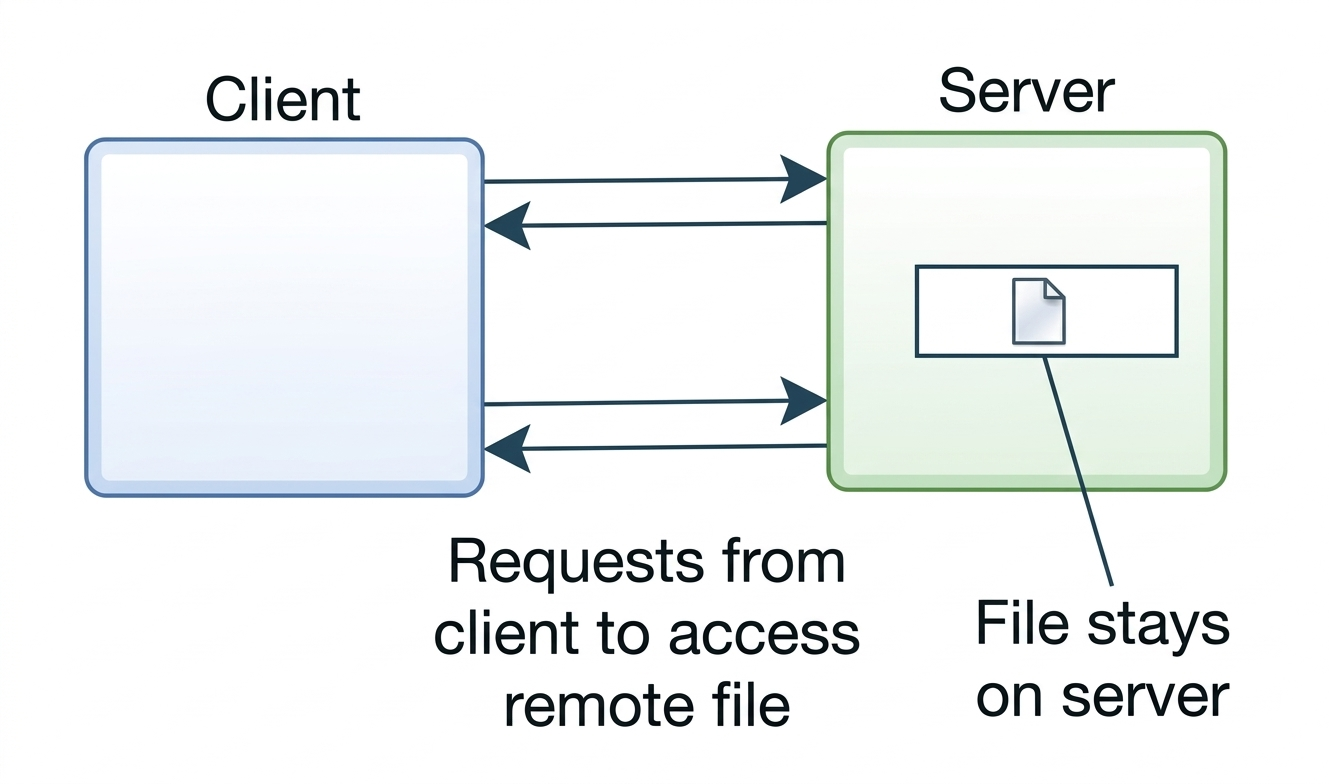
\includegraphics[width=0.5\linewidth]{fig/NetworkModels/client_server.jpg}
        \caption{Diagrama de alto nível do modelo de acesso remoto cliente-servidor, baseado em \citep{Tanenbaum2007}.}
        \label{fig:tannenbaum_client_server}
\end{figure}

\subsection{Modelo Peer-to-Peer}
\label{sec:p2p_model}

A arquitetura P2P caracteriza-se pela distribuição das responsabilidades entre os participantes da rede, sem papéis fixos de cliente e servidor. Dessa forma, um mesmo nó pode atuar tanto como provedor quanto como consumidor de serviços ao longo da comunicação. Apesar do uso amplo dessa arquitetura, não existe uma definição única para sistemas P2P, e a literatura apresenta diferentes interpretações, que variam conforme as características consideradas essenciais para esse modelo. Além disso, durante muitos anos, a arquitetura P2P foi associada ao compartilhamento de conteúdo ilegal. Essa associação, entretanto, decorre das aplicações desenvolvidas sobre essa arquitetura, e não do modelo arquitetural em si.

De acordo com a definição proposta no RFC (\textit{Request for Comments}) 5694 \citep{RFC5694}, um sistema P2P caracteriza-se pelo compartilhamento de recursos entre seus participantes para prover o serviço para o qual foi projetado. Nessa definição, os pares devem tanto fornecer serviços a outros participantes quanto requisitar serviços deles, e contribuem coletivamente para o funcionamento do sistema.

Diversos autores, como \citep{Milojicic2002}, apresentam o modelo cliente-servidor como uma arquitetura centralizada e o modelo P2P como uma arquitetura descentralizada. Essa distinção, entretanto, não constitui uma separação absoluta: conforme discutido na Seção~\ref{sec:network_architecture_models}, sistemas classificados como P2P podem conter componentes centralizados \citep{RFC5694}. A Figura~\ref{fig:centralized_vs_p2p} ilustra a comparação entre os dois modelos.


\begin{figure}[!ht]
        \centering
        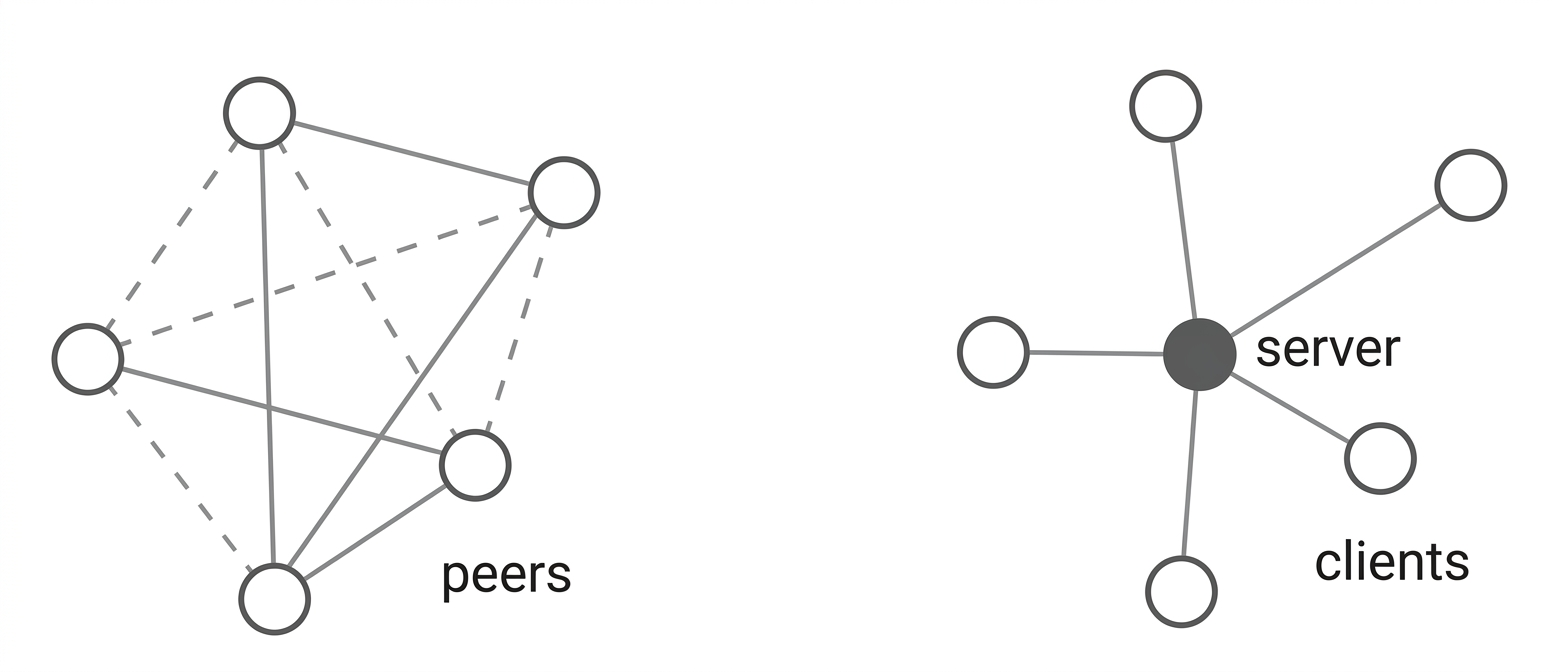
\includegraphics[width=0.6\linewidth]{fig/NetworkModels/centralized_vs_p2p.jpg}
        \caption{Diagrama de alto nível da comparação entre os modelos P2P e centralizado, baseado em \citep{Milojicic2002}.}
        \label{fig:centralized_vs_p2p}
\end{figure}

\subsection{Modelo Peer-to-Peer Híbrido}
\label{sec:hybrid_peer_to_peer_model}

Modelos P2P híbridos combinam características das arquiteturas cliente-servidor e P2P e, portanto, não pertencem exclusivamente a nenhuma delas. Nesses modelos, a comunicação principal ocorre entre os pares, porém determinadas funcionalidades, como autenticação, descoberta de pares, sinalização ou obtenção de metadados necessários à conexão, dependem de um servidor central \citep{Milojicic2002}.

A Figura~\ref{fig:hybrid_p2p} apresenta um exemplo desse modelo. Na Figura~\ref{fig:hybrid_p2p}(a), um \textit{peer} arbitrário A comunica-se com um servidor para obter as informações necessárias à conexão. Em seguida, conforme a Figura~\ref{fig:hybrid_p2p}(b), o \textit{peer} A utiliza essas informações para estabelecer uma comunicação direta com um \textit{peer} arbitrário B.

\begin{figure}[!ht]
        \centering
        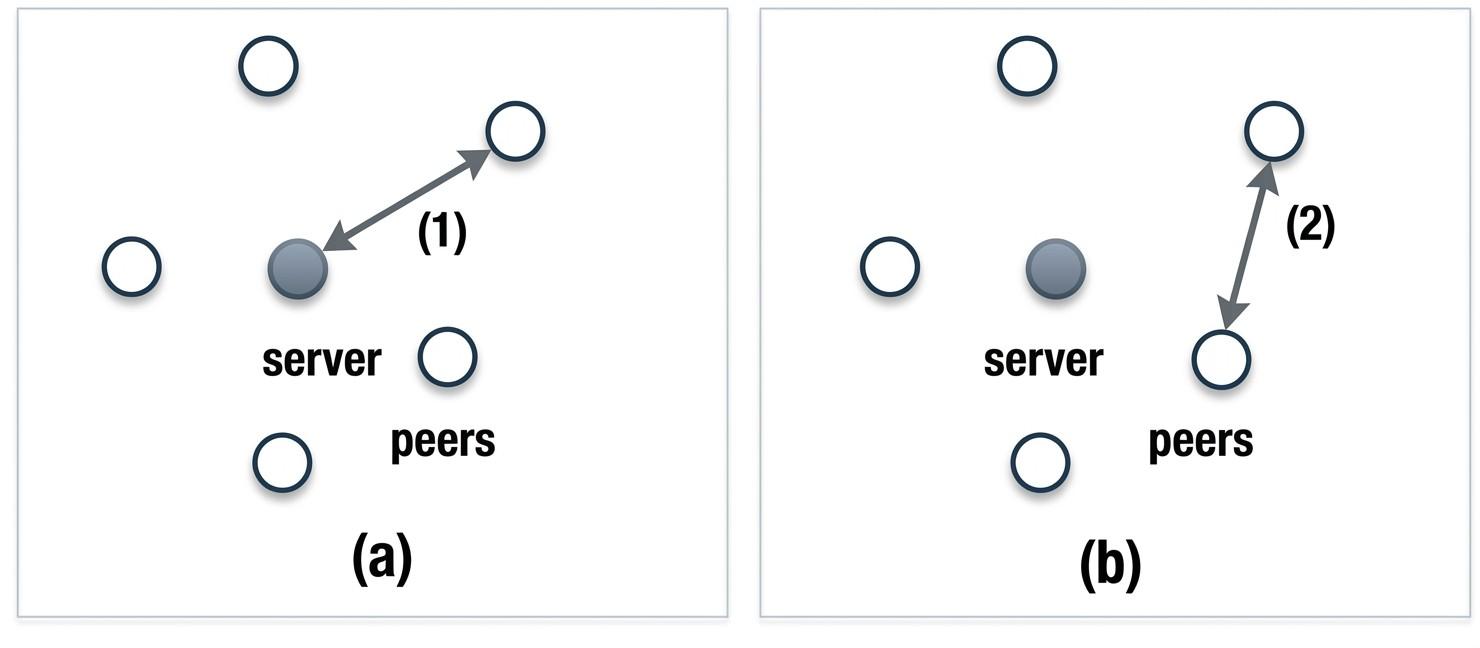
\includegraphics[width=0.6\linewidth]{fig/NetworkModels/hybrid_model.jpg}
        \caption{Exemplo de modelo híbrido, baseado em \citep{Milojicic2002}.}
        \label{fig:hybrid_p2p}
\end{figure}

\subsection{WebRTC como referência arquitetural}
\label{sec:webrtc}

O WebRTC (\textit{Web Real-Time Communication}) permite a comunicação de áudio, vídeo e dados entre \textit{peers}, tendo sido desenvolvido inicialmente para aplicações de comunicação em tempo real entre navegadores \citep{RFC8825}. Sua organização constitui um exemplo do modelo de arquitetura híbrida apresentado na Seção~\ref{sec:hybrid_peer_to_peer_model}: serviços auxiliares participam do estabelecimento da conexão, enquanto os dados podem ser transportados diretamente entre os participantes. Quando a comunicação direta não é possível, o transporte pode utilizar servidores de retransmissão (\textit{relay}).

A Figura~\ref{fig:webrtc_architecture} apresenta uma visão geral dessa arquitetura, destacando os participantes e os serviços envolvidos no estabelecimento da comunicação.

\begin{figure}[!ht]
        \centering
        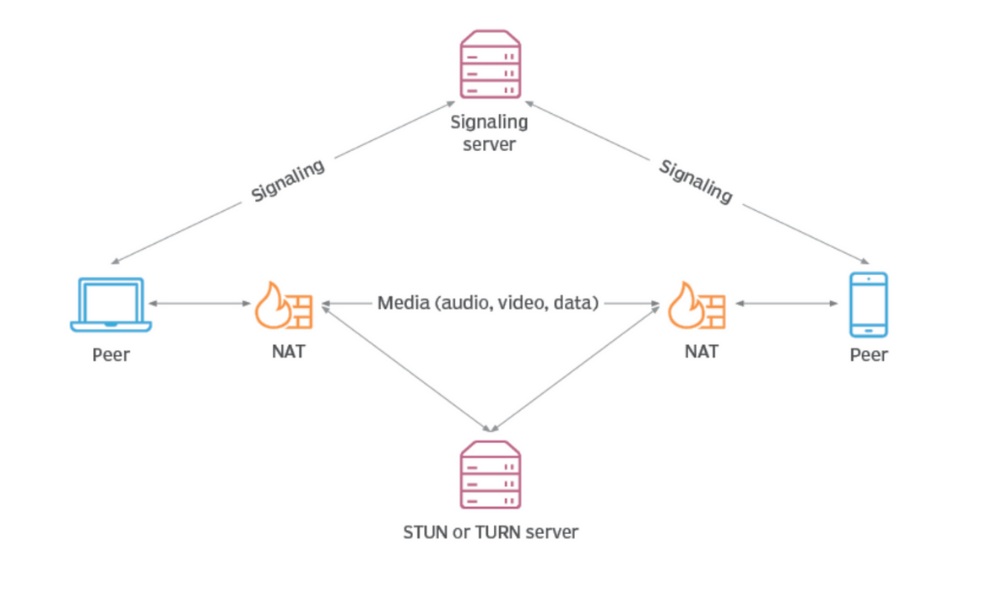
\includegraphics[width=1.0\linewidth]{fig/WebRTC/webrtc_architecture.png}
        \caption{Visão geral da arquitetura do WebRTC, conforme \citep{nugroho2026webrtcwebsocket}.}
        \label{fig:webrtc_architecture}
\end{figure}

DuBois e Ivov \citep{WebRTCForTheCurious} organizam o funcionamento do WebRTC em quatro etapas conceituais:

\begin{itemize}
    \item \textbf{Sinalização (\textit{signaling}):} troca das informações necessárias para que os participantes possam estabelecer a conexão e negociar as características da comunicação. O WebRTC não determina o mecanismo de transporte das mensagens de sinalização, cuja escolha cabe à aplicação.

    \item \textbf{Conexão (\textit{connecting}):} descoberta dos caminhos disponíveis entre os participantes e verificação de sua conectividade. Essa etapa permite selecionar um caminho direto ou retransmitido, conforme as condições das redes envolvidas.

    \item \textbf{Segurança (\textit{securing}):} estabelecimento dos mecanismos de autenticação e proteção criptográfica utilizados na comunicação entre os participantes.

    \item \textbf{Comunicação (\textit{communicating}):} transmissão dos dados das aplicações pelo caminho estabelecido, utilizando os mecanismos de proteção negociados.
\end{itemize}

Essa divisão permite distinguir as responsabilidades envolvidas na comunicação, sem exigir que cada etapa corresponda a um componente isolado. A sinalização viabiliza a troca inicial de informações, a conexão determina o caminho disponível e os mecanismos de segurança e transporte permitem a comunicação protegida entre os participantes.

Neste trabalho, o WebRTC serve como referência arquitetural para a organização dessas responsabilidades, especialmente nas etapas de sinalização e estabelecimento de conectividade entre os \textit{gateways}. A solução utiliza ICE, descrito na Seção~\ref{sec:ice}, para descobrir e selecionar os caminhos de comunicação, e QUIC, apresentado no Capítulo~\ref{chap:quic}, para transportar os dados das aplicações TCP locais e integrar os mecanismos de segurança ao estabelecimento da conexão. A proposta não utiliza a pilha completa ou a API de navegador do WebRTC.

%%%%%%%%%%%%%%%%%%%%%%%%%%%%%%%%%%%%%%%%%%%%%%%%%%%%%%%%
%%%%%%%%%%%%%%%%%%%%%%%%%%%%%%%%%%%%%%%%%%%%%%%%%%%%%%%%
%%%%%%%%%%%%%%%%%%%%%%%%%%%%%%%%%%%%%%%%%%%%%%%%%%%%%%%%
\section{Network Address Translator (NAT)}
\label{sec:network_address_translator}

O NAT é um mecanismo que traduz endereços IP entre diferentes domínios de endereçamento, como uma rede local (LAN, do inglês \textit{Local Area Network}) e uma rede de longa distância (WAN, do inglês \textit{Wide Area Network}). Essa tradução permite que a comunicação entre \textit{hosts} ocorra de forma transparente, sem que os dispositivos finais precisem conhecer ou gerenciar as alterações realizadas pelo dispositivo NAT. Conforme descrito em \citep{RFC1631}, o NAT surgiu principalmente como solução para dois problemas associados ao crescimento da Internet baseada no protocolo IPv4 (\textit{Internet Protocol version 4}): o esgotamento de endereços e a escalabilidade do sistema de roteamento.

\begin{itemize}
\item \textbf{Esgotamento de endereços:} O protocolo IPv4 utiliza endereços de 32 bits, o que permite aproximadamente 4,3 bilhões de endereços distintos. Entretanto, com a expansão da Internet e o aumento do número de dispositivos conectados, esse espaço de endereçamento mostrou-se insuficiente para atender à demanda global.

\item \textbf{Escalabilidade de roteamento:} O crescimento da Internet também aumentou a quantidade de redes e prefixos que precisam ser anunciados e armazenados pelos roteadores da infraestrutura global. A fragmentação do espaço de endereçamento aumenta o tamanho das tabelas de roteamento, o que eleva os requisitos de memória, processamento e atualização dos roteadores responsáveis pelo encaminhamento de pacotes.

\end{itemize}

\subsection{Características em Comum de NATs}

Os diferentes tipos de NAT variam quanto ao modo de realizar as traduções. Entretanto, conforme definido em \citep{RFC2663}, um mecanismo NAT deve apresentar algumas características fundamentais, implementadas de forma completa ou parcial:

\begin{itemize}
\item \textbf{Tradução transparente de endereços:} Os \textit{hosts} envolvidos na comunicação não devem precisar conhecer a existência do NAT nem as traduções realizadas, e devem operar como se a tradução não existisse.

\item \textbf{Encaminhamento transparente através da tradução:} O dispositivo NAT deve encaminhar os pacotes após a tradução de endereços de forma que, para os \textit{hosts} envolvidos, a comunicação ocorra da mesma maneira que ocorreria sem o NAT.

\item \textbf{Tradução do conteúdo de mensagens de erro ICMP:} As mensagens de erro do ICMP (\textit{Internet Control Message Protocol}) carregam em seu conteúdo uma cópia do pacote IP que originou o erro. Como essa cópia pode conter endereços ou informações de transporte modificados pelo NAT, o dispositivo deve traduzir esses campos para que o \textit{host} interno associe corretamente a mensagem de erro à conexão original.

\end{itemize}

Cabe destacar que, no RFC 1631 \citep{RFC1631}, o NAT traduz apenas endereços, enquanto definições posteriores, como a do RFC 3022 \citep{RFC3022}, introduzem o conceito de NAPT (\textit{Network Address Port Translation}), que também traduz portas.

A redução do uso de endereços IP baseia-se no pressuposto de que nem todos os dispositivos de uma rede privada precisam de um endereço IP público. Por isso, o RFC 1631 discute a necessidade de particionar o espaço de endereçamento entre endereços reutilizáveis (locais) e endereços globalmente únicos, sem, no entanto, definir faixas concretas para essa alocação. Em vez disso, o documento remete à alocação proposta no RFC 1597 \citep{rfc1597}. Posteriormente, o RFC 1918 \citep{rfc1918} tornou obsoleto o RFC 1597, manteve as mesmas faixas reservadas e as formalizou como \textit{Best Current Practice}. A Figura~\ref{fig:priv_pub_net_p2pnat} ilustra a relação entre endereços IP públicos e privados.

\begin{figure}[!ht]
        \centering
        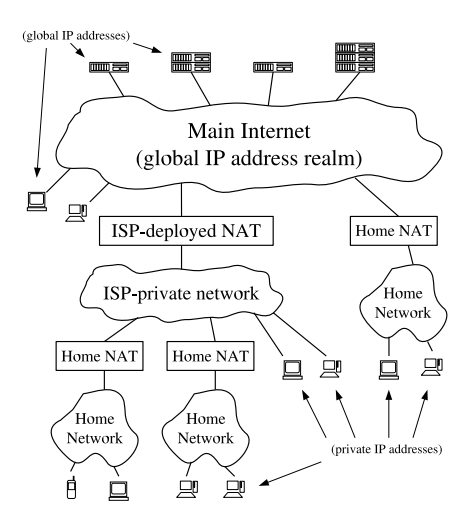
\includegraphics[width=0.5\linewidth]{fig/NATs/priv_pub_net_p2pnat.png}
        \caption{Domínios de endereços IP público e privado por \citep{ford2005peer}.}
        \label{fig:priv_pub_net_p2pnat}
\end{figure}

Entretanto, a reutilização das mesmas faixas de endereços privados em diferentes redes gera sobreposição de endereços: um mesmo endereço privado pode identificar dispositivos distintos em redes diferentes. Essa sobreposição impede que dois dispositivos situados em redes privadas distintas se comuniquem diretamente por meio de seus endereços privados \citep{RFC1631}. Esse problema é central para este trabalho, e a Seção~\ref{sec:nat_problem_for_p2p_communication} o aborda em detalhe.

\subsection{Tipos de NAT}

A literatura classifica os NATs segundo critérios distintos. Para fins de clareza, este trabalho organiza essas classificações em dois eixos: o primeiro relaciona-se ao que é traduzido, e o segundo, ao comportamento da operação de tradução. O primeiro eixo corresponde à nomenclatura do RFC 3022 \citep{RFC3022}, que divide o NAT tradicional (\textit{Traditional NAT}) em NAT básico (\textit{Basic NAT}) e NAPT, este também denominado NAT \textit{overload} ou PAT (\textit{Port Address Translation}). O segundo eixo corresponde à classificação em quatro tipos (\textit{Full Cone}, \textit{Restricted Cone}, \textit{Port-Restricted Cone} e \textit{Symmetric}), definida originalmente no RFC 3489 \citep{RFC3489}. Posteriormente, o RFC 5389 \citep{RFC5389} tornou obsoleto o RFC 3489 e abandonou essa classificação, pois muitos NATs reais não se enquadram de forma precisa em nenhum dos quatro tipos. Em seu lugar, os RFCs 4787 \citep{RFC4787} e 5780 \citep{RFC5780} adotam uma terminologia comportamental mais precisa.

\subsubsection{Classificação de NATs por Tipo de Tradução}
\label{sec:nat_classification_by_translation_type}

O RFC 3022 \citep{RFC3022} amplia o conceito original de tradução do RFC 1631. Enquanto o RFC 1631 prevê a tradução apenas do endereço IP, com mapeamento unívoco (1:1) entre um endereço local e um endereço global, o RFC 3022 formaliza o NAPT, no qual o NAT traduz múltiplos endereços locais, combinados com suas respectivas portas TCP/UDP, para um único endereço público e os diferencia pela porta atribuída. Essa abordagem decorre da necessidade de economizar endereços IPv4 públicos, cada vez mais escassos, e permite que múltiplos dispositivos de uma rede privada compartilhem simultaneamente um único endereço público.

Assim, o RFC 3022 define os seguintes tipos de tradução:
\begin{itemize}
    \item \textbf{\textit{Basic NAT}:} Tradução de endereço (mapeamento 1:1).
    \item \textbf{NAPT:} Tradução de endereço e porta (mapeamento N:1).
\end{itemize}

Além da diferenciação entre \textit{Basic NAT} e NAPT, o RFC 3022 define, de forma ortogonal a essa classificação, o modo de estabelecimento do mapeamento de tradução. No mapeamento estático, a associação entre uma identidade interna e uma identidade global é definida previamente e permanece fixa, o que permite que determinado \textit{host} ou serviço interno utilize sempre o mesmo endereço e a mesma porta globais.

No mapeamento dinâmico, por outro lado, o NAT cria os mapeamentos sob demanda, à medida que os \textit{hosts} da rede privada iniciam comunicações externas. No \textit{Basic NAT}, esse processo implica a alocação temporária de endereços globais aos endereços locais, enquanto no NAPT o dispositivo associa pares de endereço e porta internos a um par de endereço e porta externo disponível.

Dessa forma, o RFC 3022 estabelece dois modos de vinculação (\textit{binding}) aplicáveis tanto ao \textit{Basic NAT} quanto ao NAPT:
\begin{itemize}
    \item \textbf{\textit{Static NAT}:} Associação fixa e predefinida entre uma identidade privada e uma identidade global.
    \item \textbf{\textit{Dynamic NAT}:} Associação entre uma identidade privada e uma identidade global, estabelecida sob demanda a partir de um conjunto disponível.
\end{itemize}

Algumas fontes não normativas tratam o \textit{static} NAT e o \textit{dynamic} NAT como características exclusivas do \textit{Basic NAT}; entretanto, o RFC 3022 não estabelece essa restrição.

\subsubsection{Classificação de NATs por Comportamento de Tradução}
\label{sec:nat_classification_by_translation_behavior}

Os documentos de referência descrevem a classificação comportamental de NATs com diferentes níveis de granularidade. Esta seção apresenta, primeiro, a classificação clássica do RFC 3489, amplamente utilizada na literatura sobre \textit{hole punching} e comunicação P2P, e, em seguida, a classificação comportamental mais recente e detalhada do RFC 4787.

\paragraph{Classificação Clássica}

Além de definir o protocolo STUN e mecanismos de travessia de NAT, abordados nas Seções~\ref{sec:nat_traversal} e~\ref{sec:ice}, o RFC 3489 descreve uma classificação inicial dos tipos de NAT. Embora essa nomenclatura tenha se tornado obsoleta, ela permanece amplamente utilizada por motivos didáticos, e este trabalho a adota. Ainda assim, para manter a coerência com a terminologia atual, este trabalho apresenta, na sequência, as definições mais recentes.

O RFC 3489 trata apenas do NAPT, e não do \textit{Basic NAT}. Entretanto, é possível inferir que os tipos de NAT descritos a seguir se aplicam de forma semelhante ao \textit{Basic NAT}, com exceção do \textit{Symmetric} NAT, que exigiria um endereço externo distinto para cada destino. Como o NAPT estende o \textit{Basic NAT} e predomina nas redes atuais, este trabalho concentra-se no NAPT.

Com o objetivo de padronizar a nomenclatura, o RFC 3489 propõe uma classificação simples dos tipos de NAT observados na prática:

\begin{itemize}
    \item \textbf{\textit{Full Cone} NAT:} O NAT cria um único mapeamento para cada combinação de endereço e porta internos e mantém sempre o mesmo endereço e a mesma porta externos associados. Após a criação desse mapeamento, qualquer \textit{host} externo pode enviar pacotes para o endereço e a porta públicos atribuídos, independentemente de comunicação prévia com esse \textit{host}.
    \item \textbf{\textit{Restricted Cone} NAT:} Assim como no \textit{Full Cone}, uma mesma origem interna é sempre associada ao mesmo mapeamento externo. Entretanto, o recebimento de tráfego externo é restrito: apenas \textit{hosts} externos cujo endereço IP o dispositivo interno já tenha contatado podem enviar pacotes de volta através do mapeamento existente.
    \item \textbf{\textit{Port Restricted Cone} NAT:} Apresenta o mesmo comportamento do \textit{Restricted Cone}, porém a restrição também considera a porta de origem do \textit{host} externo. Dessa forma, o NAT aceita um pacote externo somente se ele tiver origem no mesmo endereço IP e na mesma porta previamente contatados pelo \textit{host} interno.
    \item \textbf{\textit{Symmetric} NAT:} O mapeamento depende não apenas do endereço e da porta internos, mas também do destino externo. Assim, uma mesma origem interna pode receber diferentes associações externas ao se comunicar com diferentes destinos. Além disso, somente o \textit{host} externo que recebeu o pacote originado pelo dispositivo interno pode enviar tráfego de volta através desse mapeamento.
\end{itemize}

Embora não exista uma definição formal padronizada, a literatura e documentações técnicas \hl{[citar exemplo]} empregam com frequência o termo \textit{Asymmetric NAT} (ou \textit{permissive NAT}) para designar, de forma genérica, todos os tipos de NAT que não são \textit{Symmetric}, ou seja, os três tipos de \textit{Cone} NAT. Este trabalho entende que essa assimetria decorre do fato de o mapeamento, conceito formalizado na classificação comportamental apresentada a seguir, depender apenas de um lado da comunicação (a origem). No \textit{Symmetric} NAT, por outro lado, o mapeamento depende do conjunto completo de endereço e porta de origem e de destino e, portanto, associa-se a um fluxo de comunicação específico: cada fluxo distinto gera um mapeamento diferente.

\paragraph{Classificação Comportamental}

Para compreender as descrições dos documentos mais recentes, é necessário entender o funcionamento de um NAPT. Conforme o RFC 4787 \citep{RFC4787}, ao receber o primeiro pacote de uma nova conexão ou de um novo fluxo, o NAPT cria em sua tabela interna (tabela NAT) uma entrada que associa o endereço e a porta internos de origem a um endereço e uma porta externos. O comportamento do NAT na criação e na reutilização desse mapeamento, bem como na filtragem de pacotes externos, determina a permissividade da tradução.

O RFC 4787 descreve esse comportamento a partir de dois eixos ortogonais: o comportamento de mapeamento (\textit{Mapping Behavior}), que define se o NAT reutiliza o mapeamento entre endereço e porta internos e externos para diferentes destinos, e o comportamento de filtragem (\textit{Filtering Behavior}), que define quais pacotes externos o NAT aceita através de um mapeamento existente. A combinação desses dois eixos caracteriza completamente um NAT e substitui, com maior granularidade, a classificação fechada em quatro tipos apresentada anteriormente.

\subparagraph{Comportamento de Mapeamento}

\begin{itemize}
    \item \textbf{\textit{Endpoint Independent Mapping} (EIM):} O NAT reutiliza o mesmo mapeamento externo para toda tradução originada da mesma tupla de endereço e porta internos, independentemente do endereço e da porta de destino.
    \item \textbf{\textit{Address Dependent Mapping} (ADM):} O NAT reutiliza o mesmo mapeamento externo para traduções originadas da mesma tupla de endereço e porta internos, desde que o pacote seja destinado ao mesmo endereço externo, independentemente da porta de destino.
    \item \textbf{\textit{Address and Port Dependent Mapping} (APDM):} O NAT reutiliza o mesmo mapeamento externo apenas para traduções originadas da mesma tupla de endereço e porta internos e destinadas à mesma tupla de endereço e porta externos.
\end{itemize}

\subparagraph{Comportamento de Filtragem}

\begin{itemize}
    \item \textbf{\textit{Endpoint Independent Filtering} (EIF):} O NAT encaminha ao \textit{host} interno qualquer pacote destinado ao endereço e à porta públicos mapeados na tabela NAT, independentemente do \textit{host} externo de origem, mesmo que o \textit{host} interno nunca tenha se comunicado com esse \textit{host} externo.
    \item \textbf{\textit{Address Dependent Filtering} (ADF):} O NAT encaminha ao \textit{host} interno apenas os pacotes que, destinados ao endereço e à porta públicos mapeados na tabela NAT, tenham origem em um endereço externo para o qual o \textit{host} interno já enviou pacotes, independentemente da porta externa de origem.
    \item \textbf{\textit{Address and Port Dependent Filtering} (APDF):} O NAT encaminha ao \textit{host} interno apenas os pacotes que, destinados ao endereço e à porta públicos mapeados na tabela NAT, tenham origem exatamente no endereço e na porta externos para os quais o \textit{host} interno já enviou pacotes.
\end{itemize}

\subsubsection{Problema do NAT para comunicações P2P}
\label{sec:nat_problem_for_p2p_communication}

Embora o NAT ofereça os benefícios, ainda que temporários, descritos na Seção~\ref{sec:network_address_translator} \citep{RFC1631}, o mecanismo impõe limitações à comunicação P2P, cuja demanda, segundo \citep{ford2005peer}, tenderia a crescer com a popularização de aplicações como VoIP (\textit{Voice over IP}) e jogos \textit{online}.

Alguns dos documentos citados apresentam o aumento de privacidade e de segurança como benefícios do NAT. Entretanto, o RFC 5128 \citep{rfc5128}, com base na Seção 2.2 do RFC 4941 \citep{RFC4941}, observa que essa privacidade é ilusória na maioria dos casos de uso de NATs em pequenos escritórios e residências (SOHO, do inglês \textit{Small-Office-Home-Office}).

A principal dificuldade que o NAT impõe às redes P2P decorre da sobreposição de endereços IP, já relatada no RFC 1631, somada ao fato de esses endereços serem privados e não roteáveis \citep{ford2005peer}. Segundo \citep{ford2005peer}, a arquitetura geral da Internet adequa-se bem ao modelo cliente-servidor, no qual dispositivos atrás de NAT apenas iniciam conexões de saída para servidores públicos conhecidos, mas pouco se adequa a modelos P2P, nos quais ambos os lados da comunicação podem estar atrás de um NAT, sem endereço público conhecido \textit{a priori}.

Embora o NAT esteja associado principalmente ao IPv4, o mesmo problema pode ocorrer no IPv6 (\textit{Internet Protocol version 6}). Conforme o RFC 5128 \citep{rfc5128}, alguma forma de NAT pode ser necessária durante a transição para o IPv6, para permitir a comunicação entre nós exclusivamente IPv4 e nós exclusivamente IPv6. O NAT-PT (\textit{Network Address Translation -- Protocol Translation}) \citep{RFC2766} tratou originalmente esse cenário, mas o RFC 4966 \citep{RFC4966} o reclassificou como histórico devido a problemas não resolvidos em sua especificação. Mecanismos mais recentes de tradução entre IPv4 e IPv6 incluem o NAT64 \citep{rfc6146} e o 464XLAT \citep{rfc6877}, e mecanismos de tradução entre endereços IPv6 incluem o NPTv6 (\textit{IPv6-to-IPv6 Network Prefix Translation}) \citep{rfc6296} e o NAT66, este ainda em proposta preliminar (\textit{Internet-Draft}) do IETF (\textit{Internet Engineering Task Force}) \citep{draft-mrw-nat66}.

Além disso, a filtragem realizada por \textit{firewalls} persistiria mesmo em um ambiente puramente IPv6, sem necessidade de tradução, e interferiria igualmente no funcionamento de aplicações P2P \citep{rfc5128}.

Diante desses problemas, surgiram métodos de travessia de NAT para viabilizar a comunicação P2P entre dispositivos atrás de NAT. Ford et al. \citep{ford2005peer} demonstram que essa travessia é viável na maioria dos casos práticos: em 380 relatos que abrangem NATs de 68 fabricantes, 82\% dos casos testados suportaram \textit{hole punching} sobre UDP, e 64\%, sobre TCP. Posteriormente, o RFC 5128 \citep{rfc5128} consolidou essas técnicas e tornou-se o documento de referência para as abordagens de travessia de NAT discutidas nas seções seguintes.

Na arquitetura proposta, esse problema afeta os gateways, que podem estar em redes privadas distintas e precisam estabelecer a comunicação externa sem depender de endereçamento público diretamente atribuído a cada host.

\section{NAT Traversal}
\label{sec:nat_traversal}

A travessia de NAT (\textit{NAT traversal}) consiste no conjunto de técnicas que viabilizam a comunicação em uma arquitetura P2P mesmo quando cada \textit{peer} está atrás de um dispositivo NAT. O RFC 5128 \citep{rfc5128} descreve os tipos mais comuns dessas técnicas desenvolvidos até a data de sua publicação.

Novas técnicas surgiram desde então, e este trabalho aborda algumas delas, como o protocolo ICE (Seção~\ref{sec:ice}) e o \textit{hole punching} com QUIC (Seção~\ref{sec:quic_hole_punching}). Entretanto, o problema e os fundamentos das soluções permanecem os mesmos, pois as limitações e a falta de padronização no comportamento dos NATs persistem.

Por conveniência de notação, esta seção emprega o termo ``endereço IP público'', salvo indicação contrária, para designar o par completo de endereço IP e porta públicos mapeados por um NAT, e não apenas o endereço IP isoladamente. Essa simplificação justifica-se porque, no NAPT (Seção~\ref{sec:nat_classification_by_translation_type}), a combinação de endereço e porta identifica de forma única um mapeamento de tradução; assim, a porta é um componente indissociável do endereço público de um \textit{peer} para fins de comunicação P2P.

\subsection{Relaying}

O \textit{relaying}, ou retransmissão, é, segundo o RFC 5128 \citep{rfc5128}, a técnica mais confiável e, ao mesmo tempo, a menos eficiente para a comunicação P2P. Em vez de estabelecer uma comunicação direta entre os dois \textit{peers}, essa técnica utiliza um servidor intermediário (\textit{Rendezvous Server}) para encaminhar os pacotes. Esse servidor realiza o registro, a descoberta e o encaminhamento de pacotes entre os \textit{peers}. Para isso, o servidor precisa possuir um endereço IP público e globalmente roteável, alcançável por ambos os \textit{peers}; do contrário, o NAT impediria que ao menos um deles o acessasse.

A vantagem desse modelo é que a comunicação sempre funciona, independentemente do tipo de NAT em cada lado, desde que ambos os \textit{peers} tenham conectividade com o servidor. Em contrapartida, essa abordagem impõe custos de infraestrutura, processamento e largura de banda ao servidor. O protocolo TURN padroniza esse tipo de servidor de retransmissão (\textit{relay}). Proposto inicialmente em um \textit{Internet-Draft} \citep{draft-ietf-behave-turn-08}, o TURN foi padronizado no RFC 5766 \citep{rfc5766}, posteriormente substituído pelo RFC 8656 \citep{rfc8656}; a Seção~\ref{sec:turn_server} descreve esse protocolo. A Figura~\ref{fig:relaying_server} ilustra esse modelo.

\begin{figure}[!ht]
        \centering
        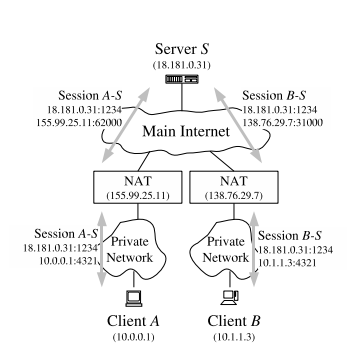
\includegraphics[width=0.5\linewidth]{fig/NAT_Traversal/relaying.png}
        \caption{Travessia de NAT por \textit{relaying}, conforme \citep{ford2005peer}.}
        \label{fig:relaying_server}
\end{figure}

\subsection{Connection Reversal}
\label{sec:connection_reversal}

O \textit{connection reversal} é uma técnica voltada para o caso em que apenas um dos \textit{peers} está atrás de um NAT (cliente A), enquanto o outro possui um endereço IP público (cliente B). O objetivo desse método é fazer com que o cliente atrás do NAT inicie a conexão com o cliente que possui endereço público, o que inverte o sentido original da tentativa de conexão. Para isso, a técnica utiliza um servidor intermediário (\textit{rendezvous point}), cuja função se limita ao registro dos \textit{peers} e à descoberta de seus respectivos endereços IP público e privado.

O processo ocorre da seguinte forma: o cliente A estabelece uma conexão com o servidor S, e o cliente B, ao se registrar, obtém por meio do servidor os endereços IP público e privado do cliente A. Em seguida, o cliente B tenta iniciar uma comunicação direta com o cliente A, utilizando ambos os endereços obtidos. Caso essa tentativa falhe, o cliente B solicita ao servidor S que encaminhe um pedido de conexão ao cliente A pela conexão já ativa entre A e o servidor. Ao receber esse pedido, o cliente A inicia uma nova conexão diretamente com o cliente B. Como o NAT permite conexões iniciadas a partir da rede interna, essa conexão será bem-sucedida desde que não haja filtragem de conexões no lado do cliente B. A Figura~\ref{fig:connection_reversal} ilustra esse processo.

\begin{figure}[!ht]
        \centering
        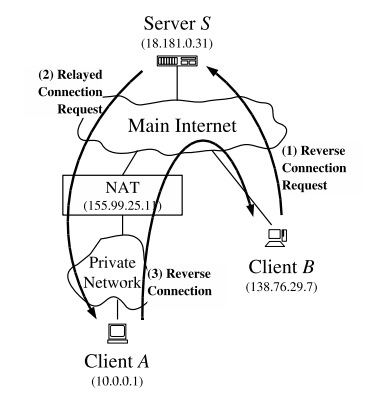
\includegraphics[width=0.5\linewidth]{fig/NAT_Traversal/connection_reversal.png}
        \caption{Travessia de NAT por \textit{connection reversal}, conforme \citep{ford2005peer}.}
        \label{fig:connection_reversal}
\end{figure}

A etapa de reversão, isto é, o encaminhamento do pedido de conexão de B para A por meio do servidor S, seguido do início da conexão por A, só ocorre caso a tentativa de conexão direta de B falhe. Se o NAT de A empregasse EIF (Seção~\ref{sec:nat_classification_by_translation_behavior}), essa tentativa direta teria sucesso para o endereço público do cliente A, e a etapa de reversão seria desnecessária.

\subsection{UDP Hole Punching}
\label{sec:udp_hole_punching}

O \textit{hole punching} sobre UDP (\textit{UDP hole punching}) é, segundo Ford et al. \citep{ford2005peer}, a técnica mais eficaz conhecida para a comunicação P2P. Essa técnica visa estabelecer a comunicação entre dois \textit{peers}, cada um atrás de um NAT, independentemente da topologia existente. Considere o seguinte cenário: dois clientes (A e B), cada um atrás de um NAT (NAT A e NAT B), e um servidor S (\textit{rendezvous server}), em que ambos os NATs são EIM e APDF. Os clientes A e B estabelecem uma sessão com o servidor S, o que cria um mapeamento A:a na tabela do NAT A e um mapeamento B:b na tabela do NAT B, em que A:a e B:b denotam os endereços públicos (endereço IP e porta) mapeados. Os clientes também obtêm, por meio do servidor, esses endereços públicos mapeados.

Caso o cliente A envie uma mensagem para B:b, o NAT B descartará os pacotes, pois o endereço IP e a porta de origem do cliente A não correspondem aos do servidor S, único \textit{host} para o qual o NAT B possui, até então, um mapeamento cuja filtragem permite a recepção de pacotes (o que não ocorreria caso o NAT B fosse EIF). Pelo mesmo motivo, o NAT A descartará as mensagens que o cliente B enviar para A:a.

Diante disso, o cliente A tenta iniciar uma sessão com o cliente B por intermédio do servidor S. O cliente A começa a enviar mensagens para B:b e, ao mesmo tempo, solicita ao servidor S que instrua o cliente B a transmitir pacotes para o endereço público A:a. Ao enviar mensagens para B:b, o cliente A faz com que o NAT A passe a aceitar, no mapeamento A:a, pacotes provenientes de B:b. Da mesma forma, ao enviar mensagens para A:a, o cliente B faz com que o NAT B passe a aceitar, no mapeamento B:b, pacotes provenientes de A:a. Com isso, os dois clientes estabelecem uma sessão direta. A Figura~\ref{fig:udp_hole_punching} ilustra esse cenário.

\begin{figure}[!ht]
        \centering
        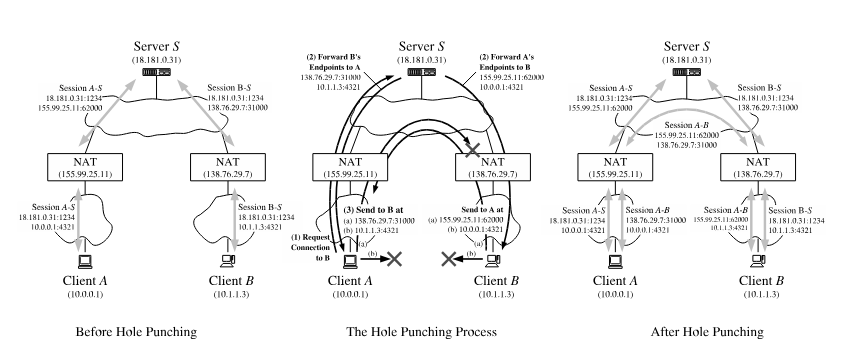
\includegraphics[width=1.0\linewidth]{fig/NAT_Traversal/udp_hole_punching.png}
        \caption{Travessia de NAT por \textit{hole punching} sobre UDP, conforme \citep{ford2005peer}.}
        \label{fig:udp_hole_punching}
\end{figure}

As técnicas de \textit{hole punching} descritas nesta seção dependem de NATs EIM; caso contrário, os clientes não conseguiriam descobrir o endereço público X:x do cliente de destino. Em NATs com mapeamento dependente do destino (EDM, do inglês \textit{Endpoint-Dependent Mapping}), isto é, ADM ou APDM, o endereço X:x seria diferente para cada destino, de modo que o servidor S não conseguiria fornecer aos clientes A e B os endereços públicos que cada um utilizaria na comunicação com o outro.

\subsubsection{UDP Hole Punching Sob o Mesmo NAT}

O \textit{hole punching} atrás do mesmo NAT corresponde ao cenário de topologia em que múltiplos \textit{peers} estão em uma mesma rede privada, sem necessariamente ter conhecimento dessa condição. Nesse cenário, duas técnicas permitem estabelecer a comunicação. Considere o cenário ilustrado na Figura~\ref{fig:udp_hole_punching_same_nat}.

Os clientes A e B inicialmente se conectam ao servidor S e obtêm seus respectivos endereços mapeados. A primeira técnica consiste em aplicar o \textit{hole punching} convencional com esses endereços públicos, o que só terá sucesso caso o dispositivo NAT suporte \textit{hairpinning}.

O \textit{hairpinning} consiste na capacidade de um NAT de encaminhar pacotes entre dois \textit{peers} da mesma rede privada quando um deles os envia ao endereço público mapeado do outro. A Figura~\ref{fig:hairpinning} ilustra esse comportamento.

\begin{figure}[!ht]
        \centering
        \hl{fazer}
 %       \includegraphics[width=1.0\linewidth]{tem que fazer}
        \caption{Técnica de NAT Hairpinning.}
        \label{fig:hairpinning}
\end{figure}

Dessa forma, quando o cliente A envia um pacote para o cliente B, o NAT traduz o endereço público B:b para o endereço privado de B, e o mesmo ocorre quando o cliente B envia um pacote para o cliente A. Entretanto, o suporte a esse comportamento está longe de ser universal: segundo Ford et al. \citep{ford2005peer}, das 335 amostras testadas para \textit{hairpin translation} em UDP, apenas 80 (24\%) o suportaram.

A segunda técnica, que independe do suporte a \textit{hairpinning}, aplica-se quando os endereços privados dos clientes são acessíveis e roteáveis entre eles. Assim como no \textit{connection reversal} (Seção~\ref{sec:connection_reversal}), os \textit{peers} informam ao servidor S tanto o endereço privado quanto o público. Ao receber os endereços do \textit{peer} de destino, cada \textit{peer} envia mensagens simultaneamente para os dois endereços, e o endereço que responder primeiro passa a ser utilizado na conexão.

\begin{figure}[!ht]
        \centering
        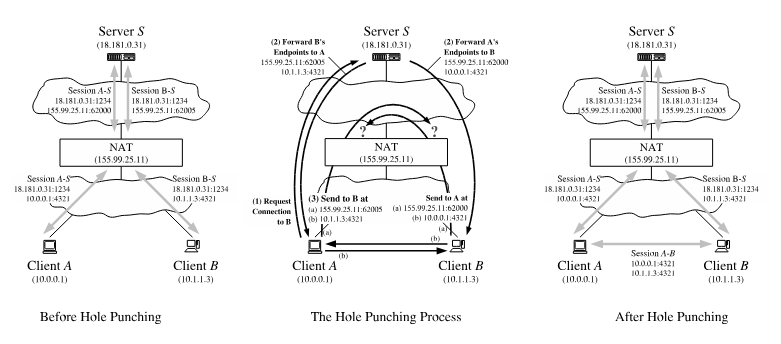
\includegraphics[width=1.0\linewidth]{fig/NAT_Traversal/udp_hole_punching_same_nat.png}
        \caption{Travessia de NAT por \textit{hole punching} sobre UDP atrás de um NAT compartilhado, conforme \citep{ford2005peer}.}
        \label{fig:udp_hole_punching_same_nat}
\end{figure}

\subsubsection{UDP Hole Punching Sob Múltiplos NATs}

Um cenário especialmente relevante na prática, dada a disseminação do \textit{Carrier-Grade NAT} (CGNAT) entre provedores de acesso à Internet (ISP, do inglês \textit{Internet Service Provider}), é o de topologias com múltiplos NATs, descrito no RFC 5128 \citep{rfc5128} e ilustrado na Figura~\ref{fig:udp_hole_punching_multiple_nat}.

Nesse caso, a comunicação se inicia como nas demais situações: os clientes A e B estabelecem conexão com o servidor S. Idealmente, o servidor S conheceria os endereços mapeados pelos NATs A e B; entretanto, esses endereços são privados no domínio de endereçamento do ISP, e os únicos endereços públicos que o servidor S conhece são os do NAT C, ao qual os NATs A e B estão conectados.

Portanto, segundo o RFC 5128, os clientes não têm outra opção senão utilizar os endereços IP públicos mapeados pelo NAT C e visíveis no domínio do servidor S, o que exige que o NAT C suporte \textit{hairpinning}.

\begin{figure}[!ht]
        \centering
        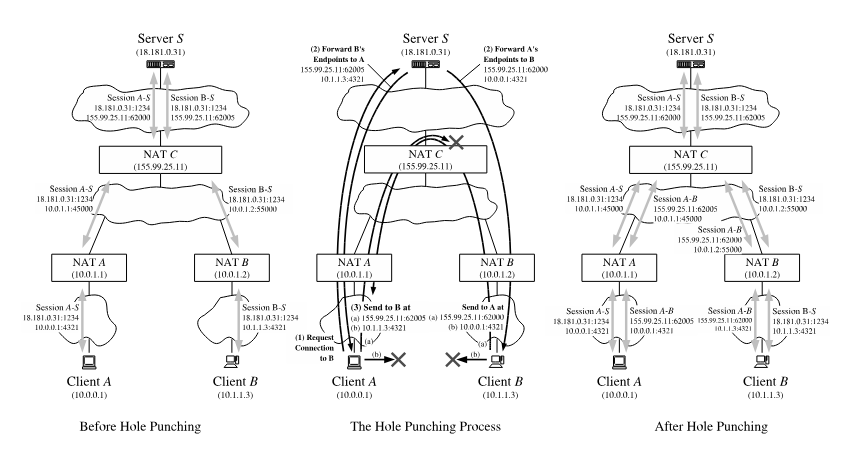
\includegraphics[width=1.0\linewidth]{fig/NAT_Traversal/udp_hole_punching_multiple_nat.png}
        \caption{Travessia de NAT por \textit{hole punching} sobre UDP atrás de múltiplos NATs, conforme \citep{ford2005peer}.}
        \label{fig:udp_hole_punching_multiple_nat}
\end{figure}

\subsubsection{UDP Hole Punching para EDM NAT}
\label{sec:udp_hole_punching_edm}

Algumas tentativas de comunicação P2P deparam-se com NATs mais restritivos, que não implementam EIM, isto é, NATs EDM (Seção~\ref{sec:nat_classification_by_translation_behavior}). Como, nesses NATs, o mapeamento público depende do destino, o servidor S não consegue informar aos \textit{peers} os endereços públicos de seus destinos.

Entretanto, conforme o RFC 5128, é possível analisar o comportamento do NAT na escolha da porta pública. Na maior parte dos casos, o NAT atribui e mapeia portas de forma sequencial, o que permite prever a próxima porta a ser alocada. Por isso, essa técnica de predição de portas (\textit{port prediction}) é frequentemente denominada ``N+1''.

Como nas seções anteriores, os clientes A e B acessam o servidor S e obtêm seus endereços públicos A:a e B:b. Em seguida, o cliente A envia mensagens para a porta prevista de B, B:b+1, e o cliente B envia mensagens para a porta prevista de A, A:a+1. Se ambos os clientes preverem corretamente a próxima porta que o NAT do outro \textit{peer} mapeará, os dois estabelecem a comunicação.

Na prática, essa técnica falha em diversos cenários: se a porta prevista já estiver em uso, se outro \textit{host} gerar um novo mapeamento antes do mapeamento da porta prevista ou se o NAT não atribuir portas de forma sequencial. Além disso, quanto mais níveis de NAT a comunicação precisar atravessar, menor a chance de sucesso, pois aumenta a probabilidade de que outro cliente envie um pacote e ocupe a porta prevista em algum dos níveis intermediários.

Por fim, para combinar essa técnica com as demais, seria necessário identificar previamente o tipo de NAT responsável pela tradução, o que aumentaria a complexidade e a latência do estabelecimento de conexão.

A predição de portas também se aplica ao \textit{hole punching} sobre TCP (Seção~\ref{sec:tcp_hole_punching}). Nesse caso, entretanto, a técnica é ainda mais frágil e sensível a \textit{timing} do que no UDP, o que torna a solução mais instável.

\subsection{TCP Hole Punching}
\label{sec:tcp_hole_punching}

O \textit{hole punching} sobre TCP (\textit{TCP hole punching}), também associado à abertura simultânea de conexões TCP (\textit{TCP simultaneous open}), segue o mesmo princípio do \textit{hole punching} sobre UDP. Entretanto, essa técnica é mais complexa devido ao problema de sincronização envolvido. Assim como no UDP, o NAT mapeia uma conexão TCP por fluxo. No UDP, que não possui o conceito de conexão, um fluxo começa com o envio do primeiro pacote e, como não há um fim explícito, o NAT remove o mapeamento, na maioria dos casos, após um tempo de inatividade (\textit{timeout}). No TCP, um fluxo começa quando o primeiro pacote \texttt{SYN} sai de um dos \textit{peers}, e seu fim é bem definido pelo envio de um pacote \texttt{FIN} ou \texttt{RST}.

O \textit{hole punching} sobre TCP também se baseia no mapeamento por fluxo da tabela NAT. Entretanto, segundo Ford et al. \citep{ford2005peer}, muitos NATs não tratam adequadamente pacotes \texttt{SYN} não solicitados. Ao receber uma conexão TCP externa, isto é, não iniciada pela rede privada, o NAT pode responder com um pacote \texttt{RST}, o que leva o NAT do remetente a remover o mapeamento do fluxo, ou simplesmente descartar o pacote. Ambos os comportamentos impedem o \textit{hole punching} sobre TCP.

Para contornar essa limitação, a técnica emprega o \textit{TCP simultaneous open}, em que ambos os \textit{peers} iniciam as conexões simultaneamente. Considere a mesma topologia da Figura~\ref{fig:udp_hole_punching}. Caso os clientes A e B enviem pacotes \texttt{SYN} ao mesmo tempo, os NATs A e B criam os mapeamentos A:a e B:b para os respectivos destinos. Assim, ao receber um pacote \texttt{SYN} logo após o envio de um \texttt{SYN} próprio, cada NAT interpreta o pacote recebido como uma resposta esperada e permite sua passagem, o que possibilita o início de uma sessão TCP. Entretanto, essa técnica não é confiável em todas as tentativas, justamente por causa da sincronização: caso um dos pacotes chegue ao NAT de destino muito antes do outro, esse NAT pode descartá-lo ou recusá-lo com um pacote \texttt{RST}. Além disso, a máquina de estados do TCP pode entrar em um estado de \textit{timeout} de fim de sessão, o que impede a aceitação de pacotes TCP mesmo que os dois \textit{peers} enviem pacotes \texttt{SYN} consecutivos.

Apesar dessas limitações, Ford et al. \citep{ford2005peer} e o RFC 5128 \citep{rfc5128} afirmam que a maior parte dos NATs permite o \textit{hole punching} sobre TCP por meio do \textit{TCP simultaneous open}, com sucesso em mais de 50\% dos casos. Ford et al. relatam, a partir de testes em uma ampla variedade de NATs, uma taxa de sucesso de 64\%. O RFC 5128 destaca ainda que outros trabalhos, com técnicas mais sofisticadas do que as de Ford et al., obtiveram suporte de até 88\% para o \textit{hole punching} sobre TCP.

\section{Interactive Connectivity Establishment (ICE)}
\label{sec:ice}

O protocolo ICE \citep{rfc8445} realiza a travessia de NAT em comunicações baseadas em UDP. O ICE utiliza o protocolo STUN e, como alternativa (\textit{fallback}), sua extensão TURN para permitir a comunicação entre dois \textit{peers}, cada um atrás de um NAT, por meio da técnica de \textit{hole punching} ou através de servidores \textit{relay}. Antes de descrever o funcionamento do ICE, as subseções a seguir apresentam os mecanismos dos protocolos STUN e TURN.

\subsection{Servidor STUN}
\label{sec:stun_server}

O STUN é um protocolo que outros protocolos utilizam para realizar a travessia de NAT; por si só, ele não constitui uma técnica de travessia, mas uma ferramenta. O STUN fornece o endereço IP e a porta que um NAT alocou para um dispositivo, permite verificar a conectividade entre \textit{endpoints} e atua como mecanismo de \textit{keep-alive}, que mantém ativos os mapeamentos da tabela NAT.

O campo de tipo das mensagens STUN divide-se em dois subcampos: a classe e o método. A classe indica a natureza da mensagem e ocupa 2 bits, o que resulta em quatro classes possíveis:

\begin{itemize}
    \item \textbf{\textit{Request}:} Mensagem que exige resposta e pode ser retransmitida;
    \item \textbf{\textit{Indication}:} Mensagem que não exige resposta;
    \item \textbf{\textit{Success Response}:} Resposta de sucesso a uma \textit{request};
    \item \textbf{\textit{Error Response}:} Resposta de erro a uma \textit{request}.
\end{itemize}

As extensões e aplicações que utilizam o STUN, como o TURN, definem, em geral, seus próprios métodos; o RFC 8489 \citep{rfc8489} define apenas o método \texttt{Binding}. Esse método retorna ao requisitante o endereço IP e a porta públicos observados pelo servidor STUN. Algumas implementações armazenam esses valores, embora o RFC 8489 não exija nem preveja esse armazenamento.

Em relação à segurança, o STUN pode operar sobre UDP, TCP, DTLS (\textit{Datagram Transport Layer Security}) sobre UDP e TLS (\textit{Transport Layer Security}) sobre TCP. Com DTLS ou TLS, a comunicação é cifrada e autenticada conforme esses protocolos. O STUN também prevê um mecanismo de autenticação por usuário e senha, com credenciais de curta ou de longa duração, aplicado a cada mensagem STUN, que pode servir como camada adicional de segurança mesmo com o uso de DTLS ou TLS. O protocolo permite essa autenticação sem DTLS ou TLS, mas essa configuração não é recomendada, pois a comunicação perde as garantias de confidencialidade providas pela criptografia dessas tecnologias.

A Figura~\ref{fig:stun_time_diagram} apresenta o diagrama de tempo do processamento de uma mensagem de método \texttt{Binding} e classe \texttt{Request}, com a respectiva resposta de método \texttt{Binding} e classe \texttt{Success Response}.

\begin{figure}[!ht]
        \centering
        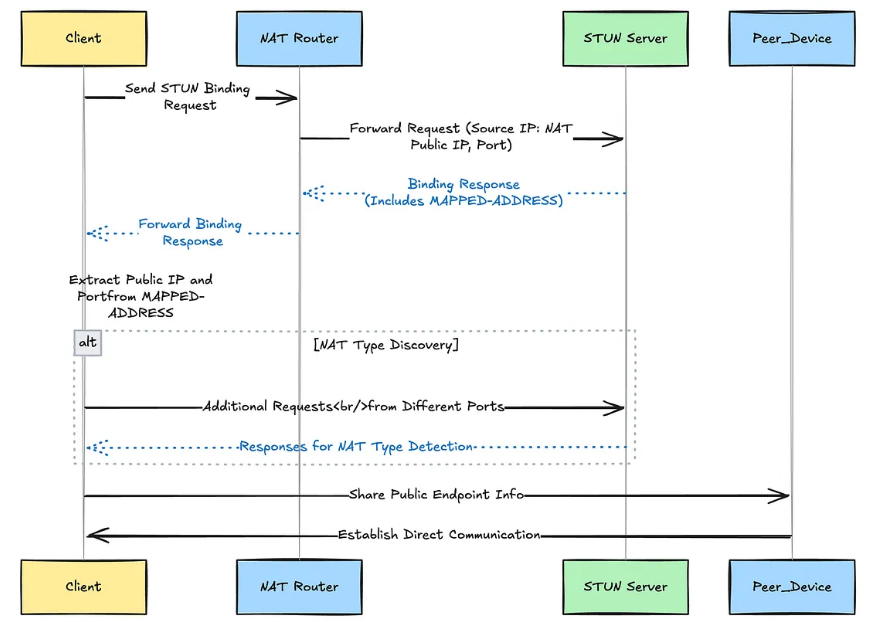
\includegraphics[width=1.0\linewidth]{fig/ICE/stun_time_diagram.png}
        \caption{Diagrama de tempo do STUN, conforme \citep{bordane2024stun}.}
        \label{fig:stun_time_diagram}
\end{figure}

\begin{comment}
CARA IMPORTANTE LEMBRAR O SEGUINTE

Hairpinning permite que de dentro da rede eu acesse o outro peer usando o IP/port público dele descober pelo STUN, isso permite que o holepunching funcione mesmo que os 2 peers estejam abaixo do mesmo NAT

Também importante lembrar onde isso se sobrepõe com aplicações UNSAF do RFC
\end{comment}

\subsection{Servidor TURN}
\label{sec:turn_server}

O TURN é um protocolo desenvolvido para viabilizar a comunicação nos casos em que dois \textit{peers} atrás de NAT não conseguem se comunicar diretamente. Esses casos, descritos nas Seções~\ref{sec:nat_classification_by_translation_behavior} e~\ref{sec:udp_hole_punching}, decorrem das limitações e dos bloqueios de NATs que não implementam EIM. Por isso, diversos trabalhos, como \citep{liao2020turnproxy}, descrevem o TURN como uma solução para os casos de falha do \textit{hole punching}.

O TURN resolve esses cenários por meio de um ponto intermediário, denominado \textit{relay} ou servidor TURN (\textit{TURN server}), que permite que \textit{peers} (\textit{TURN clients}) se comuniquem por meio de um terceiro \textit{host}. O servidor TURN também pode ocultar dos demais \textit{peers} os endereços IP e as portas públicos mapeados; nesse caso, o servidor atua como um \textit{proxy} especializado.

A Figura~\ref{fig:turn_topology} ilustra a topologia entre clientes e servidor TURN. Os clientes podem estar ou não atrás de um NAT, e cada um pode ou não atuar como \textit{TURN client}. O RFC 8656 \citep{rfc8656} define, entre outros, os seguintes endereços de transporte: o endereço do cliente no lado externo do NAT, visto pelo servidor, denomina-se \textit{server-reflexive transport address}; o endereço do servidor utilizado pelos clientes para enviar mensagens TURN denomina-se \textit{TURN server transport address}; e o endereço do \textit{peer}, visto pelo servidor, denomina-se \textit{peer transport address}.

\begin{figure}[!ht]
        \centering
        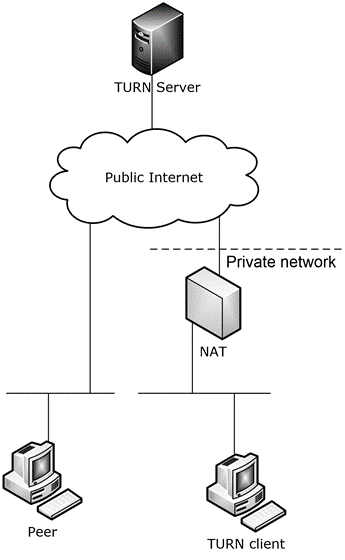
\includegraphics[width=0.4\linewidth]{fig/ICE/turn_topology.png}
        \caption{Exemplo de topologia cliente-servidor TURN, conforme \citep{microsoft2022msturn}.}
        \label{fig:turn_topology}
\end{figure}

O TURN foi projetado para operar como parte do protocolo ICE. Além disso, o TURN é uma extensão do protocolo STUN, e suas mensagens utilizam o formato das mensagens STUN.

Durante a comunicação, as mensagens enviadas de um cliente TURN ao servidor trafegam sobre um protocolo de transporte previamente escolhido. Ao receber um pacote a ser retransmitido, o servidor o desencapsula e o envia ao \textit{peer} de destino em um datagrama UDP. No sentido contrário, ao receber um datagrama UDP do \textit{peer}, o servidor TURN encapsula a mensagem em uma mensagem TURN e a encaminha ao cliente. A Tabela~\ref{tab:turn_transports} resume essa relação.

\begin{table}[htbp]
    \centering
    \begin{tabular}{|l|l|}
        \hline
        \textbf{Cliente TURN $\rightarrow$ Servidor TURN} &
        \textbf{Servidor TURN $\rightarrow$ \textit{Peer}} \\
        \hline
        UDP & UDP \\
        \hline
        TCP & UDP \\
        \hline
        TLS-over-TCP & UDP \\
        \hline
        DTLS-over-UDP & UDP \\
        \hline
    \end{tabular}
    \caption{Protocolos de transporte do TURN, conforme \citep{rfc8656}.}
    \label{tab:turn_transports}
\end{table}

Os clientes solicitam alocações ao servidor TURN por meio de uma requisição \texttt{Allocate}. O servidor autentica essas requisições com o mecanismo de autenticação do STUN e, em resposta, reserva um endereço próprio, denominado \textit{relayed transport address}. Esse endereço passa a ser o ponto de contato pelo qual os \textit{peers} enviam tráfego ao cliente, e o servidor encaminha ao cliente os dados recebidos nesse endereço. A Figura~\ref{fig:turn_time_diagram} apresenta o diagrama de tempo do processo de alocação em um servidor TURN.

\begin{figure}[!ht]
        \centering
        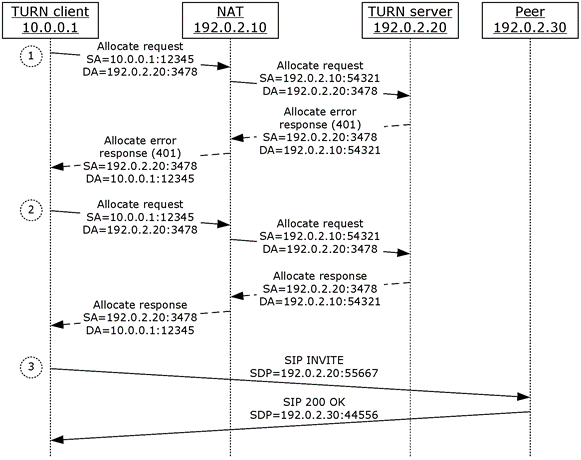
\includegraphics[width=0.8\linewidth]{fig/ICE/turn_time_diagram.png}
        \caption{Diagrama de tempo do TURN, conforme \citep{microsoft2022msturnexamples}.}
        \label{fig:turn_time_diagram}
\end{figure}

Para garantir a segurança e impedir o uso do TURN para contornar (\textit{bypass}) \textit{firewalls}, o servidor implementa o conceito de permissões: antes de aceitar tráfego de um \textit{peer} específico endereçado ao \textit{relayed transport address} do cliente, o servidor exige que o cliente tenha instalado explicitamente uma permissão para esse \textit{peer}. Esse conceito é análogo ao comportamento de filtragem dos NATs (Seção~\ref{sec:nat_classification_by_translation_behavior}). Cada permissão funciona como uma concessão temporária (\textit{lease}) e expira após 5 minutos caso o cliente não a renove.

O servidor TURN oferece dois mecanismos de envio e retransmissão de dados:

\begin{itemize}
    \item \textbf{\textit{Indications}:} As \textit{indications} são mensagens no formato STUN, conforme a Seção~\ref{sec:stun_server}, e dividem-se em dois tipos: \textit{Send Indication} e \textit{Data Indication}. A \textit{Send Indication} transporta dados do cliente ao servidor, que os retransmite ao \textit{peer}; a \textit{Data Indication} transporta ao cliente os dados que o servidor recebeu do \textit{peer};
    \item \textbf{\textit{Channels}:} Os canais utilizam um formato simplificado de mensagem, denominado \textit{ChannelData}, que dispensa o cabeçalho STUN e reduz o consumo de banda. Para criar um canal, o cliente envia uma requisição \texttt{ChannelBind} que associa um número de canal de 2 bytes, escolhido pelo próprio cliente, a um \textit{peer} específico; esse número, somado a um campo de tamanho de 2 bytes, forma o cabeçalho de 4 bytes de cada mensagem \textit{ChannelData}. O canal opera nos dois sentidos (do cliente ao \textit{peer} e do \textit{peer} ao cliente) e permanece ativo por 10 minutos caso o cliente não o renove, o dobro da duração de uma permissão, o que garante que o canal não expire antes dela.
\end{itemize}

\subsection{Protocolo ICE}

O protocolo ICE, definido no RFC 8445 \citep{rfc8445}, combina as vantagens das técnicas de travessia de NAT apresentadas anteriormente, de modo a reduzir a complexidade e maximizar o uso de comunicações P2P em diferentes topologias. O ICE opera nativamente sobre fluxos de dados (\textit{streams}) em UDP, utiliza os protocolos STUN e TURN na seleção de endereços e suporta \textit{hosts} com um ou múltiplos endereços IP (\textit{multihomed}).

O ICE baseia-se na coleta de endereços candidatos para a comunicação entre os dois \textit{peers}; cada combinação de candidatos representa uma possível tentativa de comunicação. Esses candidatos incluem o endereço local do \textit{host} (ou \textit{gateway}) e os endereços obtidos por meio dos protocolos auxiliares do ICE (STUN e TURN). A Figura~\ref{fig:ice_candidates} ilustra esses candidatos. Cada \textit{gateway} executa seu próprio agente ICE. Os candidatos obtidos e os pares selecionados referem-se aos caminhos de comunicação desses \textit{gateways}, e não aos endereços dos sensores ou atuadores associados a eles.

\begin{figure}[!ht]
        \centering
        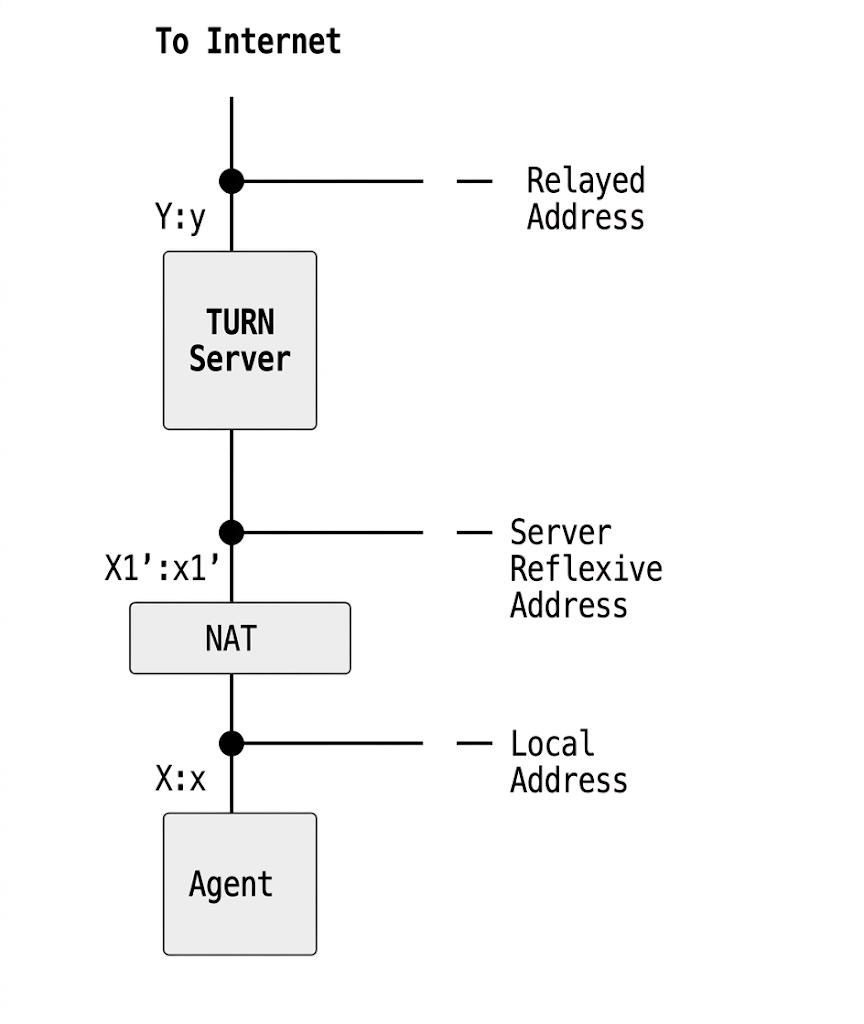
\includegraphics[width=0.6\linewidth]{fig/ICE/ice_addresses.png}
        \caption{Endereços de candidatos ICE, baseado em \citep{rfc8445}.}
        \label{fig:ice_candidates}
\end{figure}

Os candidatos apresentados na figura são:

\begin{itemize}
    \item \textbf{\textit{Local Address}:} Endereço IP da interface de rede do \textit{host};
    \item \textbf{\textit{Server Reflexive Address}:} Endereço IP público que o NAT atribui ao \textit{host}, obtido por meio do STUN;
    \item \textbf{\textit{Relayed Address}:} Endereço IP que o servidor TURN (\textit{relay}) aloca para o \textit{host}.
\end{itemize}

Há ainda o \textit{Peer Reflexive Address}, que corresponde ao endereço do \textit{host} observado pelo outro \textit{peer} e que pode diferir dos endereços observados pelos servidores STUN e TURN. O ICE descobre esse endereço durante as verificações de conectividade (\textit{connectivity checks}) e o adiciona à lista de candidatos. Em resumo, o ICE busca descobrir o maior número possível de endereços capazes de representar um \textit{peer}, a fim de encontrar ao menos um que viabilize a comunicação.

Cada candidato possui um atributo denominado \textit{base}, que representa o endereço a partir do qual o agente ICE (\textit{ICE agent}) efetivamente envia pacotes ao utilizar esse candidato. Para os candidatos \textit{host}, \textit{server-reflexive} e \textit{peer-reflexive}, a base corresponde ao \textit{local address}. Para o candidato \textit{relayed}, a base é o próprio candidato, isto é, o endereço alocado pelo servidor TURN, pois é o servidor, e não o \textit{host}, quem envia os pacotes a partir desse endereço.

Após a descoberta dos candidatos, o agente ICE os ordena por prioridade e os troca com o outro \textit{peer} por meio de um servidor de sinalização. A prioridade de cada candidato resulta de uma fórmula em que cada tipo de candidato possui um peso específico. O ICE não define o servidor de sinalização, que pode ser qualquer canal confiável entre os \textit{peers}. De posse dos candidatos de ambos os lados, o agente ICE forma pares de candidatos (\textit{candidate pairs}) e inicia as verificações de conectividade por meio de mensagens STUN \texttt{Binding} (\textit{request} e \textit{response}).

O algoritmo do ICE compreende as seguintes etapas, detalhadas a seguir:

\begin{itemize}
    \item \textbf{Ordenação de candidatos:} O agente ICE ordena os pares de candidatos por prioridade;
    \item \textbf{Verificações de conectividade:} Os agentes verificam cada par de candidatos por meio de mensagens STUN \texttt{Binding}; ao receber uma requisição de verificação, o \textit{peer} responde com uma \textit{Binding Success Response}.
\end{itemize}

\subsubsection{Verificações de Conectividade do ICE}
\label{sec:ice_connectivity_checks}

As verificações de conectividade avaliam os pares de candidatos para selecionar o melhor par da lista de prioridades e confirmar que ao menos um deles viabiliza a comunicação. O uso de \textit{relay} praticamente garante a comunicação; entretanto, por ser a opção menos eficiente, os candidatos \textit{relayed} recebem a menor prioridade e funcionam como última alternativa.

As verificações de conectividade seguem um \textit{handshake} de quatro mensagens (\textit{4-way handshake}), o que corresponde a dois RTTs (\textit{Round Trip Time}), conforme ilustra a Figura~\ref{fig:connectivity_check_4way_handshake}. O agente ICE executa as verificações na ordem da lista de prioridade dos pares de candidatos, denominada \textit{checklist}. Os \textit{triggered checks} otimizam esse processo: ao receber uma verificação de um par, o agente envia imediatamente uma verificação no sentido oposto, o que acelera a descoberta de pares válidos. O agente insere os pares que passam na verificação, denominados \textit{valid pairs}, em uma lista própria, a \textit{valid list}. Ao final do processo, o ICE seleciona um par por componente; assim, há mais de um par selecionado apenas quando a comunicação possui mais de um componente de \textit{stream}, como no uso do RTP (\textit{Real-time Transport Protocol}) e do RTCP (\textit{RTP Control Protocol}), protocolos que são utilizados no padrão WebRTC descritos na Seção~\ref{sec:webrtc}, em cenários sem multiplexação de componentes (Estes protocolos podem ou não multiplexar diferentes \textit{streams} no mesmo endereço).

\begin{figure}[!ht]
        \centering
        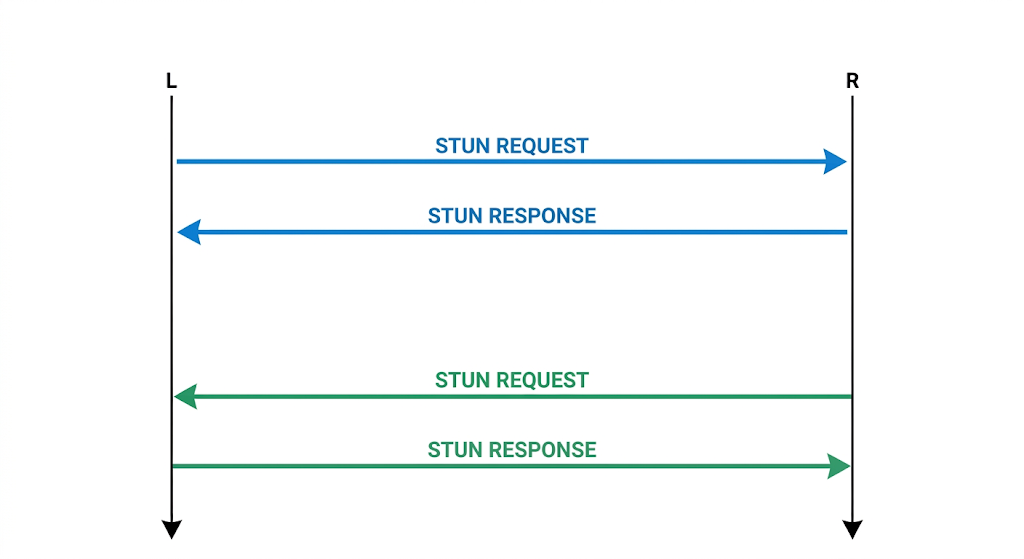
\includegraphics[width=0.7\linewidth]{fig/ICE/4way_handshake.png}
        \caption{\textit{4-way handshake} das verificações de conectividade do ICE, baseado em \citep{rfc8445}.}
        \label{fig:connectivity_check_4way_handshake}
\end{figure}

Durante as verificações de conectividade, o ICE atribui um papel a cada \textit{peer}: um atua como agente controlador (\textit{controlling agent}) e o outro, como agente controlado (\textit{controlled agent}). Essa atribuição define a condição de parada das verificações, que prosseguem até que o agente controlador encontre um par válido. Em seguida, o agente controlador envia uma requisição STUN \texttt{Binding} com o atributo \texttt{USE-CANDIDATE}, que informa ao agente controlado o par a ser utilizado para a transmissão de dados a partir desse momento (Figura~\ref{fig:4way_and_attribute}).

\begin{figure}[!ht]
        \centering
        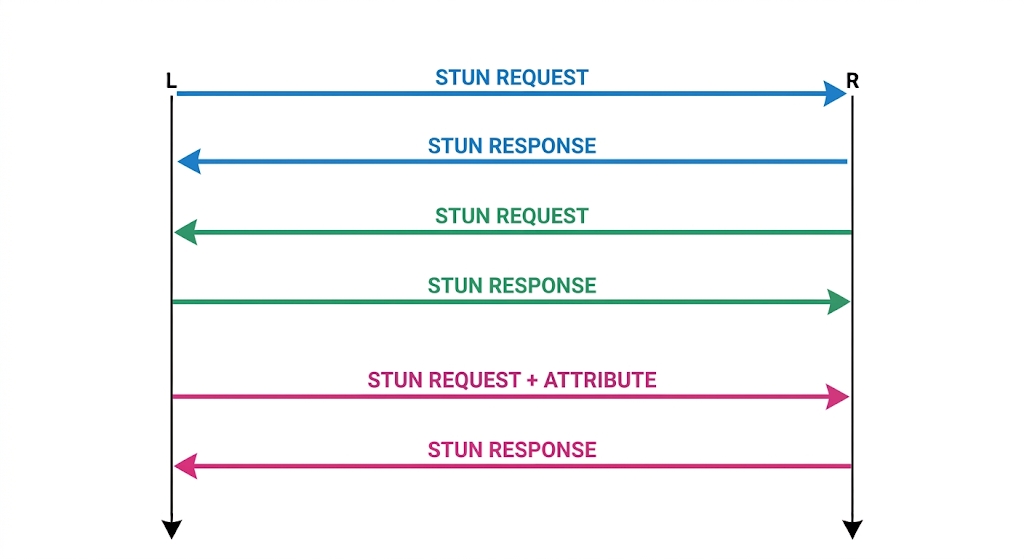
\includegraphics[width=0.7\linewidth]{fig/ICE/4way_and_attribute.png}
        \caption{\textit{4-way handshake} das verificações de conectividade do ICE com o atributo \texttt{USE-CANDIDATE}, baseado em \citep{rfc8445}.}
        \label{fig:4way_and_attribute}
\end{figure}

Como os pacotes do \textit{4-way handshake} podem ser perdidos, o agente ICE os retransmite em intervalos determinados. A perda de um pacote pode decorrer do comportamento de filtragem do NAT (Seção~\ref{sec:nat_classification_by_translation_behavior}) ou de características do meio. O primeiro motivo é o relevante, pois o ICE testa justamente a permissividade dos NATs. Portanto, para que o agente considere um par inválido apenas quando um NAT restritivo o bloqueia, a retransmissão é necessária, de modo a descartar perdas causadas por problemas de temporização, sincronização ou limitações do meio. Dois parâmetros definidos pelo protocolo, Ta e RTO (\textit{Retransmission Timeout}), regem as políticas de transmissão e retransmissão das verificações de conectividade:

\begin{itemize}
    \item \textbf{Ta:} Intervalo mínimo entre o envio de verificações de conectividade. Como pode haver mais de uma verificação em andamento, retransmissões podem ocorrer enquanto o agente gera novas verificações. O RFC 8445 sugere Ta de 50~ms, mas admite outros valores, desde que respeitem o limite mínimo de 5~ms;
    \item \textbf{RTO:} Tempo de espera antes de uma retransmissão. O protocolo STUN define esse parâmetro \citep{rfc8489}, cujo valor dobra a cada nova retransmissão. O RFC 8445 define o cálculo do RTO inicial, mas admite outros cálculos, desde que o valor inicial seja maior ou igual a 500~ms.
\end{itemize}

\section{Chownat}
\label{sec:chownat}

O Chownat é uma aplicação desenvolvida por Kamkar \citep{kamkar2004chownat} que aplica as técnicas de travessia de NAT apresentadas na Seção~\ref{sec:udp_hole_punching} para estabelecer uma conexão entre dois \textit{peers}, cada um atrás de um NAT, e encapsular tráfego TCP em UDP. Para isso, a aplicação divide os \textit{peers} em cliente e servidor: o cliente sempre inicia a conexão, e o servidor aguarda a mensagem do cliente.

\subsection{Arquitetura do Chownat}

O Chownat possui uma arquitetura que permite o tunelamento de serviços TCP sobre UDP. Para isso, a aplicação mantém abertos dois \textit{sockets}: um UDP, que realiza o \textit{hole punching}, e um TCP, que gerencia o serviço TCP. A Figura~\ref{fig:chownat_architecture} ilustra essa arquitetura.

\begin{figure}[!ht]
        \centering
        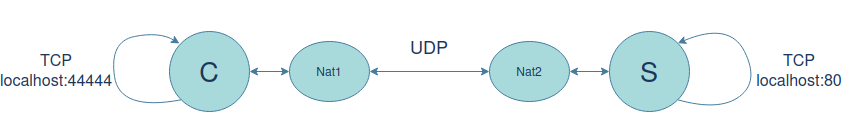
\includegraphics[width=1.0\linewidth]{fig/chownat/chownat_architecture.png}
        \caption{Diagrama de arquitetura do Chownat.}
        \label{fig:chownat_architecture}
\end{figure}

As portas indicadas na Figura~\ref{fig:chownat_architecture} são apenas ilustrativas e correspondem a um exemplo de tunelamento do tráfego TCP de um serviço HTTP (porta 80); o Chownat, entretanto, suporta qualquer serviço TCP. Este trabalho utiliza a versão 0.07 do Chownat \citep{kamkar2004chownatv07}.

O \textit{socket} UDP utiliza uma porta local escolhida e envia pacotes ao endereço IP público do \textit{peer} de destino. Para simplificar o cenário, o Chownat utiliza a mesma porta nos dois \textit{peers}, cuja porta padrão é a 2222. Essa porta é também a utilizada no \textit{hole punching}: como o Chownat não dispõe da infraestrutura de servidores e de descoberta de candidatos do ICE (Seção~\ref{sec:ice}), o endereço IP público do \textit{peer} deve ser configurado previamente, e o NAT deve preservar a porta na tradução.

Por exemplo, se o \textit{socket} UDP do cliente estiver vinculado a cIP:2222, o NAT1 precisará traduzi-lo para nat1IP:2222, de modo que o \textit{peer} servidor S consiga enviar pacotes para nat1IP:2222. Da mesma forma, o servidor terá o endereço sIP:2222, e o NAT2 precisará traduzi-lo para nat2IP:2222. Esse é o cenário necessário para que a comunicação e o \textit{hole punching} do Chownat funcionem. Com a infraestrutura de servidores do ICE, essa rigidez seria evitada, pois os endereços públicos seriam descobertos dinamicamente, e a porta pública não precisaria coincidir com a porta vinculada ao \textit{socket} UDP.

O \textit{socket} TCP vincula-se ao endereço \textit{localhost} e a uma porta que depende da função do \textit{peer}; assim, todo o tráfego TCP ocorre internamente no \textit{peer}. No servidor, a porta corresponde à do serviço associado (no exemplo da Figura~\ref{fig:chownat_architecture}, a porta 80 do serviço HTTP). No cliente, o Chownat utiliza qualquer porta livre (no exemplo, a porta 44444), para a qual o cliente do serviço TCP direciona todo o seu tráfego. Como o transporte TCP ocorre apenas localmente, o Chownat coleta o \textit{payload} (conteúdo) que o cliente TCP envia ao \textit{socket} e transporta apenas esse \textit{payload} via UDP, sem os segmentos de controle do TCP. Da mesma forma, o Chownat coleta o \textit{payload} recebido pelo \textit{socket} UDP e o entrega ao serviço local por meio do \textit{socket} TCP. Esse processo constitui o tunelamento de TCP sobre UDP.

Embora utilize técnicas associadas ao modelo P2P, o Chownat não adota necessariamente esse modelo, pois seu transporte segue a lógica cliente-servidor (Seção~\ref{sec:network_architecture_models}). Como o Chownat apenas fornece o meio de comunicação entre os \textit{peers} e não define o papel de cada nó em relação à informação transmitida, a arquitetura geral depende do serviço executado sobre ele.

\subsection{Protocolo Chownat}
\label{sec:chownat_protocol}

O protocolo do Chownat é simples e recupera pacotes perdidos por meio de pacotes de controle, além de prover as operações básicas necessárias à comunicação. O protocolo também deve viabilizar o \textit{hole punching} sobre UDP. Dessa forma, ele se divide em duas etapas: a etapa de conexão e a etapa de comunicação. Antes de descrevê-las, esta seção apresenta o cabeçalho e os tipos de pacotes utilizados.

\subsubsection{Tipos de Pacote do Chownat}

O Chownat utiliza dois tipos de pacotes, de controle e de dados, que compartilham o mesmo formato de cabeçalho. A análise do código-fonte da versão 0.07 \citep{kamkar2004chownatv07} indica que esse cabeçalho possui 3 bytes, no formato ilustrado na Figura~\ref{fig:header_chownat}.

\begin{figure}[!ht]
        \centering
        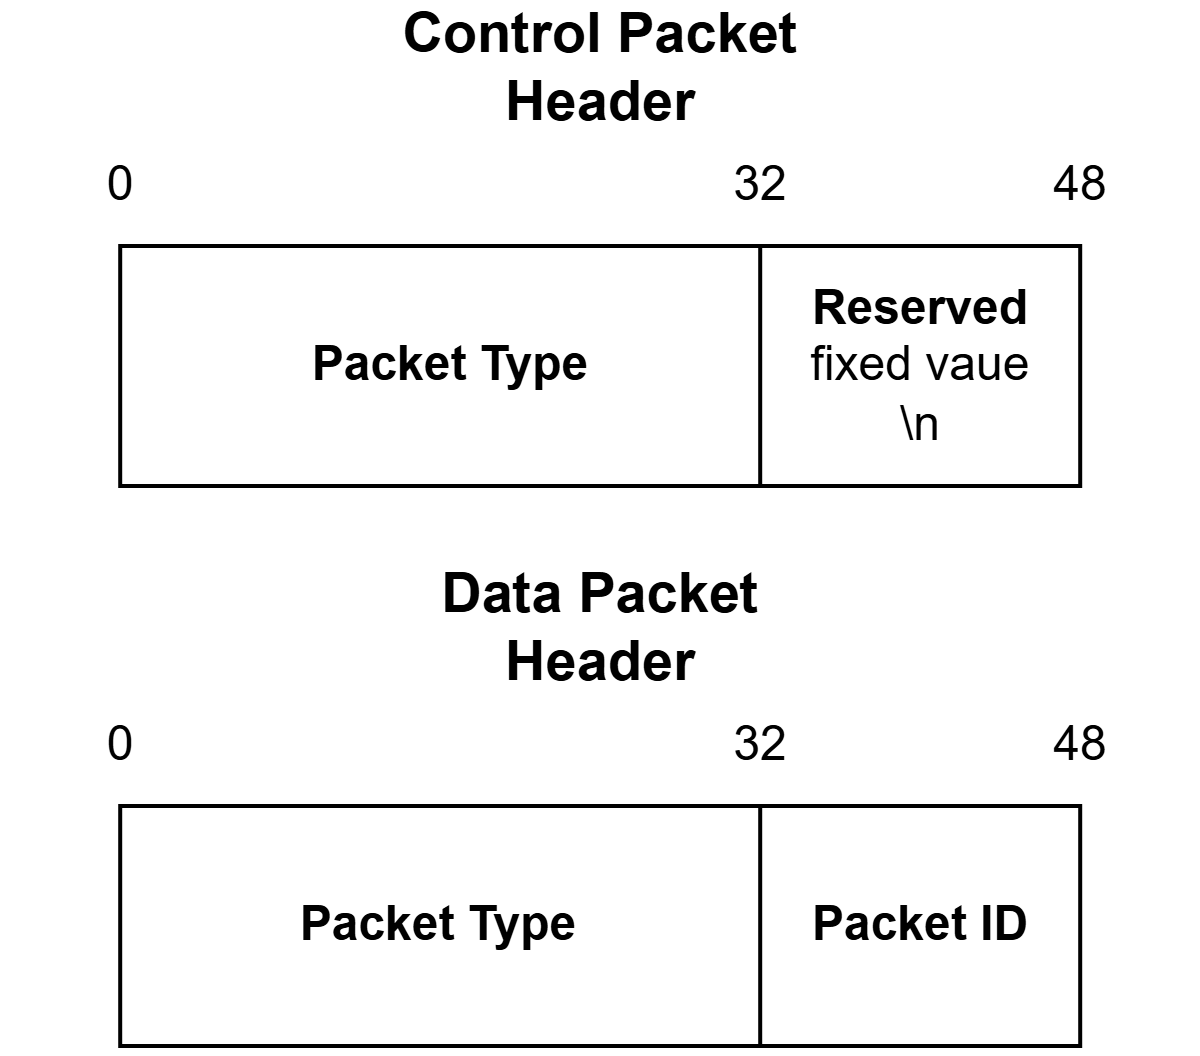
\includegraphics[width=0.6\linewidth]{fig/chownat/chownat_headers.png}
        \caption{Cabeçalhos do Chownat.}
        \label{fig:header_chownat}
\end{figure}

O campo \textit{packet type} abrange 5 tipos de pacotes, distribuídos entre controle e dados, descritos a seguir.

\paragraph{Pacotes de Controle}

\begin{itemize}
    \item \textbf{01:} Pacote de início de conexão, que o cliente Chownat envia para iniciar uma nova conexão e o processo de \textit{hole punching};
    \item \textbf{02:} Pacote de fim de conexão, que o cliente ou o servidor Chownat envia para encerrar uma conexão;
    \item \textbf{03:} Pacote de \textit{keep-alive}, que o servidor utiliza para iniciar o processo de \textit{hole punching} e que ambos os \textit{peers} utilizam para manter o mapeamento do endereço público em seus respectivos NATs.
\end{itemize}

\paragraph{Pacotes de Dados}

\begin{itemize}
    \item \textbf{08:} Pacote de requisição de retransmissão, que ambos os \textit{peers} podem utilizar para solicitar a retransmissão de pacotes; o campo \textit{packet ID} indica a partir de qual pacote o \textit{peer} necessita da retransmissão;
    \item \textbf{09:} Pacote de envio de dados, que ambos os \textit{peers} utilizam para enviar o \textit{payload} do serviço TCP; o campo \textit{packet ID} funciona como número de sequência do pacote.
\end{itemize}

\subsubsection{Etapa de Conexão do Protocolo Chownat}
\label{sec:chownat_connection}

A etapa de conexão realiza o \textit{hole punching} e um \textit{3-way handshake} que confirma a conexão entre os dois \textit{peers}. Cada \textit{peer} segue um fluxo distinto, e a combinação das ações de ambos viabiliza a comunicação; por isso, a comunicação exige um cliente e um servidor, e não ocorre entre dois clientes ou entre dois servidores.

O servidor inicialmente vincula (\textit{bind}) os \textit{sockets} TCP e UDP e aguarda o cliente por um intervalo fixo de 5~s. Sempre que esse intervalo se esgota, o servidor envia um pacote de \textit{keep-alive}, que gera o mapeamento do fluxo de comunicação no NAT e, assim, define o endereço IP e a porta públicos. Quando o \textit{hole punching} ocorre, o servidor recebe uma requisição de conexão do cliente e inicia o \textit{3-way handshake}. Se o \textit{handshake} for bem-sucedido, o servidor conecta seu \textit{socket} TCP local ao serviço TCP desejado (no exemplo, o serviço HTTP na porta 80) e conclui a etapa de conexão.

O cliente também vincula inicialmente os \textit{sockets}; entretanto, em vez de aguardar uma mensagem, como o servidor, o cliente aguarda uma conexão TCP em \texttt{localhost:Porta Servico} e atua como servidor TCP local (na Figura~\ref{fig:chownat_architecture}, \texttt{PortaServico} corresponde à porta 44444). O cliente local do serviço (no exemplo, o cliente HTTP) inicia essa comunicação ao direcionar seu tráfego para \texttt{localhost:PortaServico}. O cliente Chownat, então, aceita a conexão TCP e tenta se conectar ao servidor Chownat. Se o servidor Chownat já tiver enviado o primeiro pacote de \textit{keep-alive} e o NAT já tiver mapeado o endereço e a porta públicos, o \textit{3-way handshake} se inicia e, se bem-sucedido, conclui a etapa de conexão.

Em síntese, no Chownat há um cliente e um servidor UDP para o \textit{hole punching}, enquanto, no TCP, os papéis se invertem: o cliente Chownat atua como servidor TCP e recebe requisições TCP externas à aplicação, e o servidor Chownat atua como cliente TCP, inicia a conexão com o serviço TCP local e redireciona a ele o conteúdo recebido nos pacotes UDP, originalmente enviado pelo cliente TCP conectado ao cliente Chownat.

\subsubsection{Etapa de Comunicação do Protocolo Chownat}

A etapa de comunicação realiza o tunelamento de dados TCP sobre UDP nos dois sentidos. No sentido cliente-servidor, o cliente Chownat coleta o \textit{payload} recebido em seu \textit{socket} TCP local, no qual atua como servidor, e o encaminha pelo túnel UDP ao servidor Chownat, que o entrega ao serviço TCP local ao qual está conectado como cliente. No sentido servidor-cliente, o servidor Chownat coleta as respostas do serviço TCP e as encaminha pelo túnel UDP ao cliente Chownat, que as entrega ao cliente TCP local. A Figura~\ref{fig:chownat_architecture} ilustra esse fluxo com o exemplo de uma requisição HTTP, detalhado a seguir.

No exemplo, o cliente HTTP no \textit{peer} do cliente Chownat envia uma requisição para \texttt{localhost:PortaServico} (porta 44444), na qual o cliente Chownat a recebe como servidor TCP local. De posse do \textit{payload} dessa requisição, o cliente Chownat o encaminha pelo túnel UDP estabelecido com o servidor Chownat ao final da etapa de conexão (Seção~\ref{sec:chownat_connection}).

Ao receber esse pacote, o servidor Chownat encaminha o \textit{payload} ao serviço HTTP local pela conexão TCP que ele próprio estabeleceu, como cliente, ao final da etapa de conexão. O Chownat continua a repassar os pacotes nesse fluxo até que uma das partes encerre a conexão: o cliente HTTP local, ao final da requisição, ou o serviço HTTP local, por qualquer motivo (pacote inválido, serviço indisponível ou outro erro).

Como cada \textit{peer} gerencia a conexão TCP localmente, os segmentos de controle do TCP não trafegam pelo túnel UDP e, portanto, não existem na rede, o que torna a troca de informações mais rápida e reduz o uso de banda. Em contrapartida, como os mecanismos de controle do TCP não atuam sobre o túnel, o próprio protocolo Chownat assume esse controle e provê as garantias possíveis, como retransmissão de pacotes e ordem de chegada.

O Chownat garante a ordem de chegada e a retransmissão de pacotes por meio de um identificador único no cabeçalho dos pacotes de dados. O receptor detecta a perda de um pacote pela chegada de um pacote fora de ordem: ao receber um pacote cujo identificador não corresponde ao próximo esperado, o receptor descarta esse pacote e solicita a retransmissão a partir do identificador esperado, o que indica a perda dos pacotes intermediários.

Por exemplo, suponha que o cliente Chownat envie três pacotes ao servidor Chownat: o primeiro chega normalmente, o segundo se perde e o terceiro chega fora de ordem. Como o identificador do terceiro pacote não corresponde ao esperado (o do segundo), o servidor descarta esse pacote e solicita a retransmissão a partir do segundo; o cliente, então, reenvia o segundo e o terceiro pacotes. Caso a perda ocorra no último pacote de uma sequência, nenhum pacote subsequente chega fora de ordem para revelar a perda, e o mecanismo do Chownat não a detecta; nesses casos, cabe ao próprio serviço TCP tunelado perceber a ausência de resposta e solicitar a retransmissão na camada de aplicação.

Para manter o mapeamento no NAT e a disponibilidade da comunicação, o Chownat utiliza as mensagens de \textit{keep-alive}. Além de servirem de base para o início da comunicação, essas mensagens impedem que o mapeamento expire por inatividade na tabela NAT. O Chownat envia um pacote de \textit{keep-alive} sempre que permanece 5~s sem receber pacotes.

O Chownat apresenta limitações. Além da perda de parte dos recursos de controle do TCP, o protocolo implementa a desconexão apenas parcialmente: embora o protocolo preveja a desconexão, a implementação original da versão 0.07 apenas entra em \textit{loop}, e uma camada superior, como o sistema operacional, precisa finalizar o processo. Assim, para executar novamente o serviço TCP, é necessário um novo processo de conexão, com nova etapa de \textit{hole punching}, o que restringe a aplicação do Chownat. Na adaptação proposta neste trabalho, as aplicações e os serviços TCP locais são executados nos hosts que representam os gateways. Essa organização fornece o ponto de integração entre os dados das aplicações locais e o transporte externo.

\begin{comment}
    
\section{Web Real-Time Communication (WebRTC)}
\label{sec:webrtc}

Segundo o RFC 8825 \citep{RFC8825}, o WebRTC é um conjunto de protocolos que permite a comunicação de áudio, vídeo e dados entre \textit{peers} pelo caminho mais curto entre eles. O padrão foi desenvolvido inicialmente para o tráfego de tempo real entre navegadores, sobretudo videochamadas, e posteriormente se estendeu a outros tipos de aplicação.

Conforme \citep{WebRTCOrg} e \citep{Sequeira2017WebRTCHistory}, o WebRTC tem origem em tecnologias da GIPS (\textit{Global IP Solutions}), empresa adquirida pelo Google em 2010, que tornou essas tecnologias abertas em 2011. Atualmente, o W3C (\textit{World Wide Web Consortium}) e o IETF mantêm o padrão com escopos distintos \citep{RFC8825}: o W3C define uma API padronizada em JavaScript para a comunicação entre navegadores, enquanto o IETF define os protocolos de forma independente dessa API, de modo que quaisquer \textit{peers} que implementem o mesmo conjunto de especificações possam se comunicar entre si.

Como seu escopo não envolve comunicação Web, este trabalho concentra-se na abordagem do IETF, sobretudo do ponto de vista arquitetural. Ainda assim, a arquitetura concebida para o tráfego Web é útil para diversos outros tipos de comunicação. Por isso, este trabalho adota como principal referência o livro de DuBois e Ivov \citep{WebRTCForTheCurious}, que privilegia os aspectos técnicos e normativos do WebRTC e, portanto, se alinha ao escopo deste projeto.

DuBois e Ivov \citep{WebRTCForTheCurious} refinam a distinção entre W3C e IETF ao propor uma divisão terminológica entre \textit{protocolo WebRTC} e \textit{API WebRTC}: o protocolo WebRTC corresponde à comunicação bidirecional entre dois \textit{peers}, enquanto a API constitui um nível de abstração sobre o protocolo que permite que desenvolvedores o utilizem. Este trabalho adota essa nomenclatura, salvo indicação contrária.

\subsection{Protocolo WebRTC}
\label{sec:webrtc_protocol}

O protocolo WebRTC compõe-se de etapas sequenciais: cada etapa só começa após a conclusão bem-sucedida da anterior, condição necessária para garantir o transporte. Segundo DuBois e Ivov \citep{WebRTCForTheCurious}, essas etapas são:

\begin{itemize}
    \item \textit{Signaling} (sinalização);
    \item \textit{Connecting} (conexão);
    \item \textit{Securing} (segurança);
    \item \textit{Communicating} (comunicação).
\end{itemize}

A Seção~\ref{sec:webrtc_architecture} descreve cada uma dessas etapas, que dependem de um ou mais protocolos para sua conclusão. Assim, o WebRTC baseia-se em um conjunto de técnicas e protocolos já consolidados. A Figura~\ref{fig:webrtc_protocols} apresenta os protocolos utilizados por um \textit{peer} WebRTC.

\begin{figure}[!ht]
        \centering
        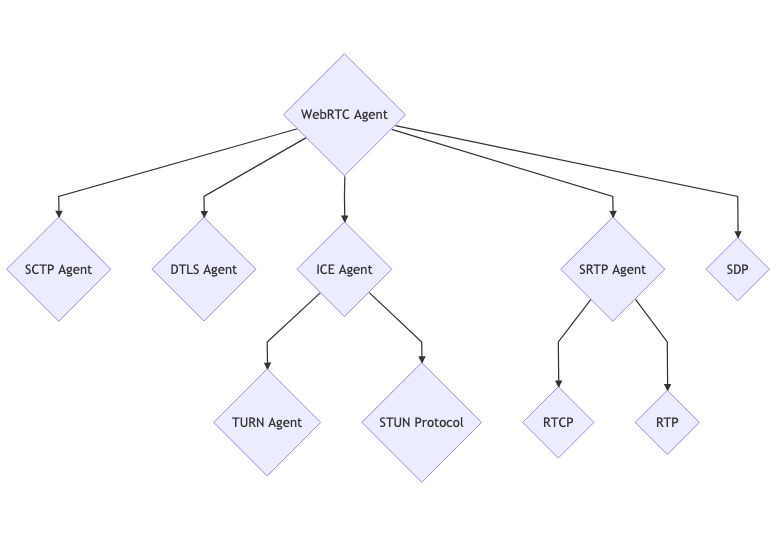
\includegraphics[width=1.0\linewidth]{fig/WebRTC/webrtc_protocol_tree.png}
        \caption{Árvore de dependência dos protocolos do WebRTC, conforme \citep{WebRTCForTheCurious}.}
        \label{fig:webrtc_protocols}
\end{figure}

\subsection{Arquitetura do WebRTC}
\label{sec:webrtc_architecture}

A arquitetura do protocolo WebRTC segue as etapas descritas na Seção~\ref{sec:webrtc_protocol} e pode ser vista, em muitos aspectos, como uma arquitetura híbrida (Seção~\ref{sec:hybrid_peer_to_peer_model}): a etapa inicial de descoberta de endereços segue o modelo cliente-servidor, enquanto a comunicação posterior entre os \textit{peers}, direta ou por meio de \textit{relay}, segue o modelo P2P. A Figura~\ref{fig:webrtc_architecture} ilustra essa arquitetura.

Neste trabalho, a arquitetura do WebRTC serve como referência para as etapas de sinalização e estabelecimento de conectividade por meio do ICE. A comunicação entre os \textit{gateways} utiliza QUIC (Capítulo~\ref{chap:quic}, que integra transporte e segurança no estabelecimento da conexão. A solução não utiliza a API WebRTC de navegador, os canais de dados SCTP ou os mecanismos de transmissão de áudio e vídeo descritos nas subseções seguintes.

\begin{figure}[!ht]
        \centering
        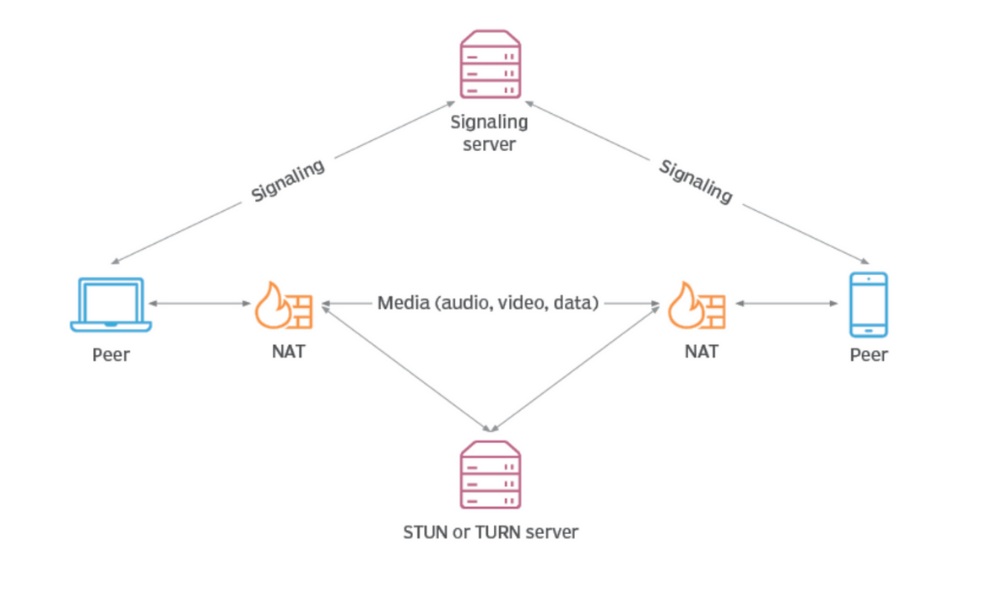
\includegraphics[width=1.0\linewidth]{fig/WebRTC/webrtc_architecture.png}
        \caption{Visão geral da arquitetura do WebRTC, conforme \citep{nugroho2026webrtcwebsocket}.}
        \label{fig:webrtc_architecture}
\end{figure}

\subsubsection{Signaling}
\label{sec:signaling}

A sinalização é a etapa inicial da conexão do protocolo WebRTC. Essa etapa é necessária porque, ao iniciar uma nova instância de conexão WebRTC, denominada agente WebRTC por DuBois e Ivov \citep{WebRTCForTheCurious}, o agente não possui nenhuma informação sobre o \textit{peer} de destino e, portanto, precisa de um meio de troca de mensagens para localizá-lo. O WebRTC não define um protocolo ou serviço para essa troca de mensagens, cuja escolha cabe à aplicação.

Para a sinalização, o protocolo WebRTC utiliza o SDP (\textit{Session Description Protocol}). Como o SDP não foi projetado especificamente para o WebRTC, esta seção não o aborda em seu escopo completo e apresenta apenas os conceitos necessários para compreender seu uso na sinalização do WebRTC.

\paragraph{SDP}

O SDP é um protocolo que padroniza a troca de informações em sessões multimídia. O RFC 2327 \citep{rfc2327} definiu originalmente o SDP, o RFC 4566 \citep{rfc4566} o revisou e, mais recentemente, o RFC 8866 \citep{rfc8866} o consolidou. O protocolo baseia-se em descritores no formato chave-valor (\texttt{<Type>=<Value>}), organizados em descritores de sessão e de mídia. Os descritores de mídia descrevem os fluxos de áudio, vídeo e dados oferecidos, com seus respectivos atributos (\textit{codecs}, credenciais do ICE, impressão digital do certificado, entre outros). A Figura~\ref{fig:sdp_example} apresenta o diagrama de fluxo do SDP.

\begin{figure}[!ht]
        \centering
        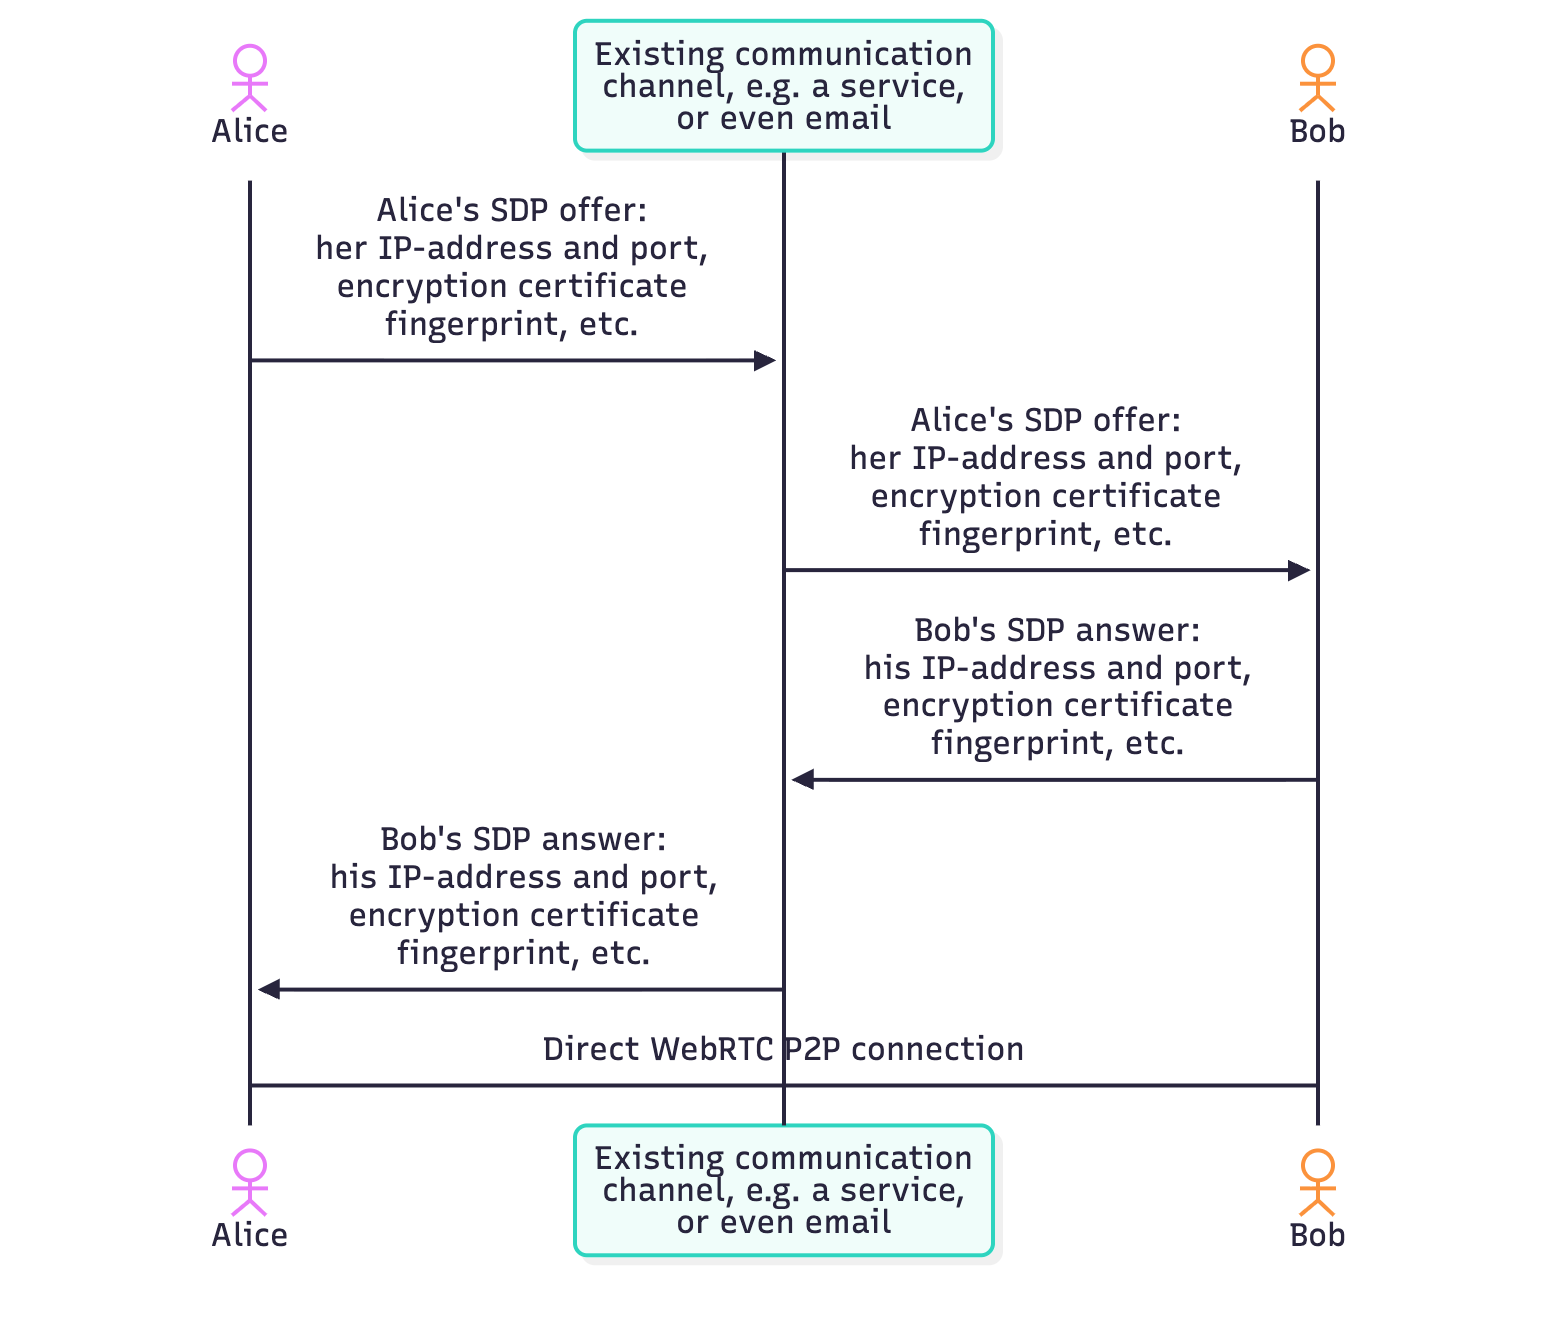
\includegraphics[width=1.0\linewidth]{fig/WebRTC/sdp_example.png}
        \caption{Diagrama de fluxo do SDP, conforme \citep{WebRTCForTheCurious}.}
        \label{fig:sdp_example}
\end{figure}

No contexto do WebRTC, os agentes utilizam o SDP segundo o modelo de oferta e resposta (\textit{offer/answer model}): um agente envia uma oferta com sua descrição de sessão, e o outro responde com uma descrição que aceita apenas os fluxos de seu interesse.

\subsubsection{Connecting}
\label{sec:connecting}

Conforme a Seção~\ref{sec:hybrid_peer_to_peer_model}, o WebRTC adota um modelo de arquitetura híbrido \citep{WebRTCForTheCurious}: emprega o modelo cliente-servidor na troca inicial de informações com os servidores STUN e TURN (Seção~\ref{sec:ice}) e, em seguida, adota o modelo P2P entre os agentes WebRTC.

A necessidade do ICE e dos servidores STUN e TURN decorre justamente da comunicação P2P, sujeita aos problemas descritos na Seção~\ref{sec:nat_problem_for_p2p_communication} e às características do NAT descritas na Seção~\ref{sec:network_address_translator}. As condições que viabilizam as técnicas de travessia no WebRTC são as mesmas descritas na Seção~\ref{sec:udp_hole_punching}.

Na prática, cada agente WebRTC coleta seus próprios candidatos (endereços locais, refletidos via STUN e, quando necessário, retransmitidos via TURN) e os troca com o agente remoto por meio dos atributos \texttt{a=candidate} da descrição de sessão (\textit{Session Description}), durante a sinalização (Seção~\ref{sec:signaling}). De posse dos candidatos de ambos os lados, o agente ICE forma pares de candidatos e testa a conectividade entre eles; os pares que trocam tráfego com sucesso tornam-se pares válidos (\textit{Valid Candidate Pairs}). Em seguida, o agente controlador escolhe um desses pares válidos e o nomeia como \textit{Nominated Pair}. Os agentes controlador e controlado realizam, então, uma última rodada de comunicação bidirecional sobre esse par; se bem-sucedida, o \textit{Nominated Pair} torna-se o \textit{Selected Candidate Pair}, utilizado durante o restante da sessão. A conclusão desse processo de seleção encerra a etapa de conexão do protocolo WebRTC. A Seção~\ref{sec:ice} detalha esse processo.

\subsubsection{Securing}
\label{sec:securing}

A segurança do protocolo WebRTC decorre da autenticação e da cifragem da conexão com o agente WebRTC remoto por meio do DTLS, em conjunto com um protocolo de comunicação como o SRTP (\textit{Secure Real-time Transport Protocol}), de modo que terceiros não tenham acesso às informações transmitidas. Entretanto, como a autenticação do DTLS depende da impressão digital do certificado trocada durante a sinalização (Seção~\ref{sec:signaling}), o protocolo não protege contra ataques \textit{man-in-the-middle} caso o canal de sinalização seja comprometido.

\paragraph{DTLS}

O DTLS \citep{RFC6347} é um protocolo projetado para ser o mais semelhante possível ao TLS, porém adaptado a datagramas. O TLS opera sobre o TCP e, portanto, depende de um transporte que garanta a entrega e a ordem dos pacotes. Como muitas aplicações passaram a utilizar o UDP e precisavam das mesmas garantias de autenticação e cifragem que o TLS oferece sobre o TCP, o IETF desenvolveu o DTLS.

Assim como o TLS, o DTLS realiza a troca das chaves utilizadas na criptografia e verifica os certificados apresentados no \textit{handshake}. No WebRTC, o agente compara o \textit{hash} do certificado apresentado durante o \textit{handshake} DTLS com a impressão digital (\textit{fingerprint}) do certificado trocada previamente via SDP, na sinalização (Seção~\ref{sec:signaling}).

\subsubsection{Communicating}
\label{sec:webrtc_communicating}

Segundo o RFC 8825 \citep{RFC8825}, a comunicação de um agente WebRTC abrange três tipos de conteúdo: áudio, vídeo e dados, cada um com características e protocolos próprios. A comunicação de áudio e vídeo ocorre em tempo real, um dos principais focos do WebRTC.

A etapa de comunicação ocorre após o estabelecimento da segurança (Seção~\ref{sec:securing}) e utiliza um protocolo de transporte. O WebRTC pode utilizar os seguintes protocolos de transporte:

\begin{itemize}
    \item \textbf{RTP e RTCP:} O RTP \citep{RFC3550} transporta informações de tempo real, como áudio e vídeo. Além dos dados, o RTP fornece números de sequência, marcas de tempo (\textit{timestamps}) e monitoramento de entrega; entretanto, não protege contra perda de pacotes nem garante a entrega em ordem ou qualquer recurso de QoS (\textit{Quality of Service}), o que exige, quando aplicável, outros protocolos que forneçam essas garantias. O RTCP constitui a camada de controle do RTP: gerencia a QoS e transmite informações sobre a sessão entre os \textit{peers}. Ambos os protocolos operam, em geral, sobre UDP;
    \item \textbf{SRTP e SRTCP:} O SRTP e o SRTCP (\textit{Secure RTCP}) \citep{RFC3711} são as versões seguras do RTP e do RTCP e garantem cifragem, autenticação e integridade. O SRTP utiliza dois níveis de chave: uma chave mestra (\textit{master key}), obtida por um mecanismo externo de estabelecimento de chaves, como o DTLS, e chaves de sessão, derivadas da chave mestra e usadas na cifragem dos dados de uma sessão. Os algoritmos utilizados incluem o AES (\textit{Advanced Encryption Standard}) em modo contador (AES-CM, \textit{Counter Mode}) e o HMAC-SHA1 (\textit{Hash-based Message Authentication Code} com \textit{Secure Hash Algorithm 1});
    \item \textbf{SCTP:} O SCTP (\textit{Stream Control Transmission Protocol}) \citep{RFC4960}, atualizado pelo RFC 9260 \citep{RFC9260}, é um protocolo de transporte que opera diretamente sobre o IP. O SCTP foi desenvolvido originalmente para transportar mensagens de sinalização de redes PSTN (\textit{Public Switched Telephone Network}) e passou a ser utilizado em aplicações mais amplas, como o WebRTC, no qual transmite dados sem requisitos de tempo real e opera encapsulado em DTLS sobre UDP. O SCTP é orientado a conexão, garante a entrega e, diferentemente do TCP, permite múltiplos fluxos (\textit{streams}) em uma mesma associação, o que evita o bloqueio de cabeça de fila (\textit{head-of-line blocking}) entre fluxos. O SCTP também oferece suporte nativo a \textit{multihoming}, isto é, a \textit{hosts} com múltiplos endereços IP e rotas disponíveis.
\end{itemize}

\subsection{WebRTC API}

A API WebRTC expõe ao desenvolvedor uma interface central, \texttt{RTCPeerConnection}, que representa a sessão WebRTC como um todo. Por meio dessa interface, o desenvolvedor adiciona fluxos de mídia com o método \texttt{addTrack}, que cria um novo fluxo RTP a ser transmitido, ou abre um canal de dados com o método \texttt{createDataChannel}, que inicializa uma associação SCTP sob demanda.

A descoberta dos endereços remotos ocorre por meio da troca de descrições de sessão. O método \texttt{createOffer} gera uma descrição do estado local do \textit{peer}, que a aplicação envia ao \textit{peer} remoto por um mecanismo externo de sinalização. Ao recebê-la, o \textit{peer} remoto a aplica e responde com uma descrição gerada pelo método \texttt{createAnswer}. Após ambos os lados aplicarem as respectivas descrições remotas, a comunicação P2P pode ser estabelecida. O método \texttt{addIceCandidate} permite incorporar, a qualquer momento, candidatos adicionais descobertos ao longo do processo.

Além disso, a API expõe um conjunto de \textit{callbacks} que notificam a aplicação sobre eventos relevantes da sessão, como o recebimento de uma nova sessão ou a mudança no estado de conectividade.

\end{comment}